%!TEX root = ../../Heun_Dale_Haney_A_dynamic_approach_to_input_output_modeling.tex
%%%%%%%%%%%%%%%%%%%%% chapter.tex %%%%%%%%%%%%%%%%%%%%%%%%%%%%%%%%%
%
% sample chapter
%
% Use this file as a template for your own input.
%
%%%%%%%%%%%%%%%%%%%%%%%% Springer-Verlag %%%%%%%%%%%%%%%%%%%%%%%%%%
%\motto{Use the template \emph{chapter.tex} to style the various elements of your chapter content.}

%%%%%%%%%%%%%%%%%%%%%%%%%%%%%%%%%%%%%%%%%%%
%%%%%%%%%% Embodied Energy Flows %%%%%%%%%%
%%%%%%%%%%%%%%%%%%%%%%%%%%%%%%%%%%%%%%%%%%%
\chapter{Embodied energy flows}
% Always give a unique label
\label{chap:embodied_energy}
% use \chaptermark{} to alter or adjust the chapter heading in the running head
\chaptermark{Embodied energy}
%%%%%%%%%%%%%%%%%%%%%%%%%%%%%%%%%%%%%%%%%%%
%%%%%%%%%%%%%%%%%%%%%%%%%%%%%%%%%%%%%%%%%%%
%%%%%%%%%%%%%%%%%%%%%%%%%%%%%%%%%%%%%%%%%%%


\abstract*{[NEED TO ADD ABSTRACT HERE]}

%% \abstract{Each chapter should be preceded by an abstract (10--15 lines long) that summarizes the content. The abstract will appear \textit{online} at \url{www.SpringerLink.com} and be available with unrestricted access. This allows unregistered users to read the abstract as a teaser for the complete chapter. As a general rule the abstracts will not appear in the printed version of your book unless it is the style of your particular book or that of the series to which your book belongs.\newline\indent
%% Please use the 'starred' version of the new Springer \texttt{abstract} command for typesetting the text of the online abstracts (cf. source file of this chapter template \texttt{abstract}) and include them with the source files of your manuscript. Use the plain \texttt{abstract} command if the abstract is also to appear in the printed version of the book.}
%% Use the template \emph{chapter.tex} together with the Springer document class SVMono (monograph-type books) or SVMult (edited books) to style the various elements of your chapter content in the Springer layout.


In Chapter~\ref{chap:direct_energy}, the 
First Law of Thermodynamics\index{First Law of Thermodynamics}
accounted direct energy ($\dot{E}$) flowing among sectors of an economy.
In this chapter, we will adapt the First Law to account  
\emph{embodied} energy\index{embodied energy}\index{energy!embodied|see{embodied energy}}
in the material flows of 
an economy.\footnote{To the authors' knowledge, 
this is the first appearance in the literature 
of a systematic, detailed, and mathematically rigorous derivation 
of embodied energy accounting equations based upon the 
laws of thermodynamics.}

Energy can become ``embodied'' in the output of an economic sector
and within the material in the sector itself.
The energy embodied in the output of an economic sector 
(e.g., energy embodied in the automobiles produced by the automotive sector)
is related to the sum of all direct energy
consumed in the manufacture of its products, 
including all upstream processing stages. 
Embodied energy gives an indication 
of the energy demand created by consumption of goods and services
within an economy.

Energy that becomes embodied in the materials of an economic sector 
(such as the machines, factories, and dealerships 
within the automotive sector itself) is essential for 
the efficient operation of the sector. The amount of energy
embodied in the sector is an indicator of the complexity of
the sector; the amount of energy embodied in an entire economy
can be an indicator of the level of 
economic development\index{economic development}
of the economy.

The purpose of this chapter is to develop a model for 
embodied energy flows within economies. 
With an embodied energy model in hand, we will be positioned
to develop a model for the energy intensity 
of goods and services within an economy 
(Chapter~\ref{chap:intensity}).


%%%%%%%%%% Embodied Energy: Methodology %%%%%%%%%%
\section{Methodology}
\label{sec:embodied_methodology}
%%%%%%%%%%

We begin the derivation of embodied energy accounting
equations by defining the concept of 
\emph{total} energy\index{total energy}\index{energy!total|see{total energy}}. 


%+++++++++ Embodied Energy: Total Energy Accounting ++++++++++
\subsection{Total energy accounting}
\label{sec:total_energy_accounting}
%+++++++++

Total energy ($T$)\nomenclature[T]{$T$}{total energy [J]}
is defined as the sum of 
direct energy\index{direct energy} 
($E$, see Chapter~\ref{chap:direct_energy}) 
and embodied energy ($B$)\nomenclature[B]{$B$}{embodied energy [J]}.

\begin{equation} \label{eq:T_def}
	T \equiv E + B
\end{equation}

The flow rate of total energy 
($\dot{T}$)\nomenclature[T]{$\dot{T}$}{total energy flow rate [W]}
among sectors in 
the economy, the biosphere, and society is the sum of
direct energy ($\dot{E}$) and embodied 
energy ($\dot{B}$)\nomenclature[B]{$\dot{B}$}{embodied energy flow rate [W]}.

\begin{equation} \label{eq:T_dot_def}
	\dot{T} = \dot{E} + \dot{B}
\end{equation}

\noindent Figure~\ref{fig:embodied_single_producer} illustrates
that total energy flows are comprised of
direct energy ($\dot{E}$) and embodied energy ($\dot{B}$). 

\begin{figure}[!ht]
	\centering\
	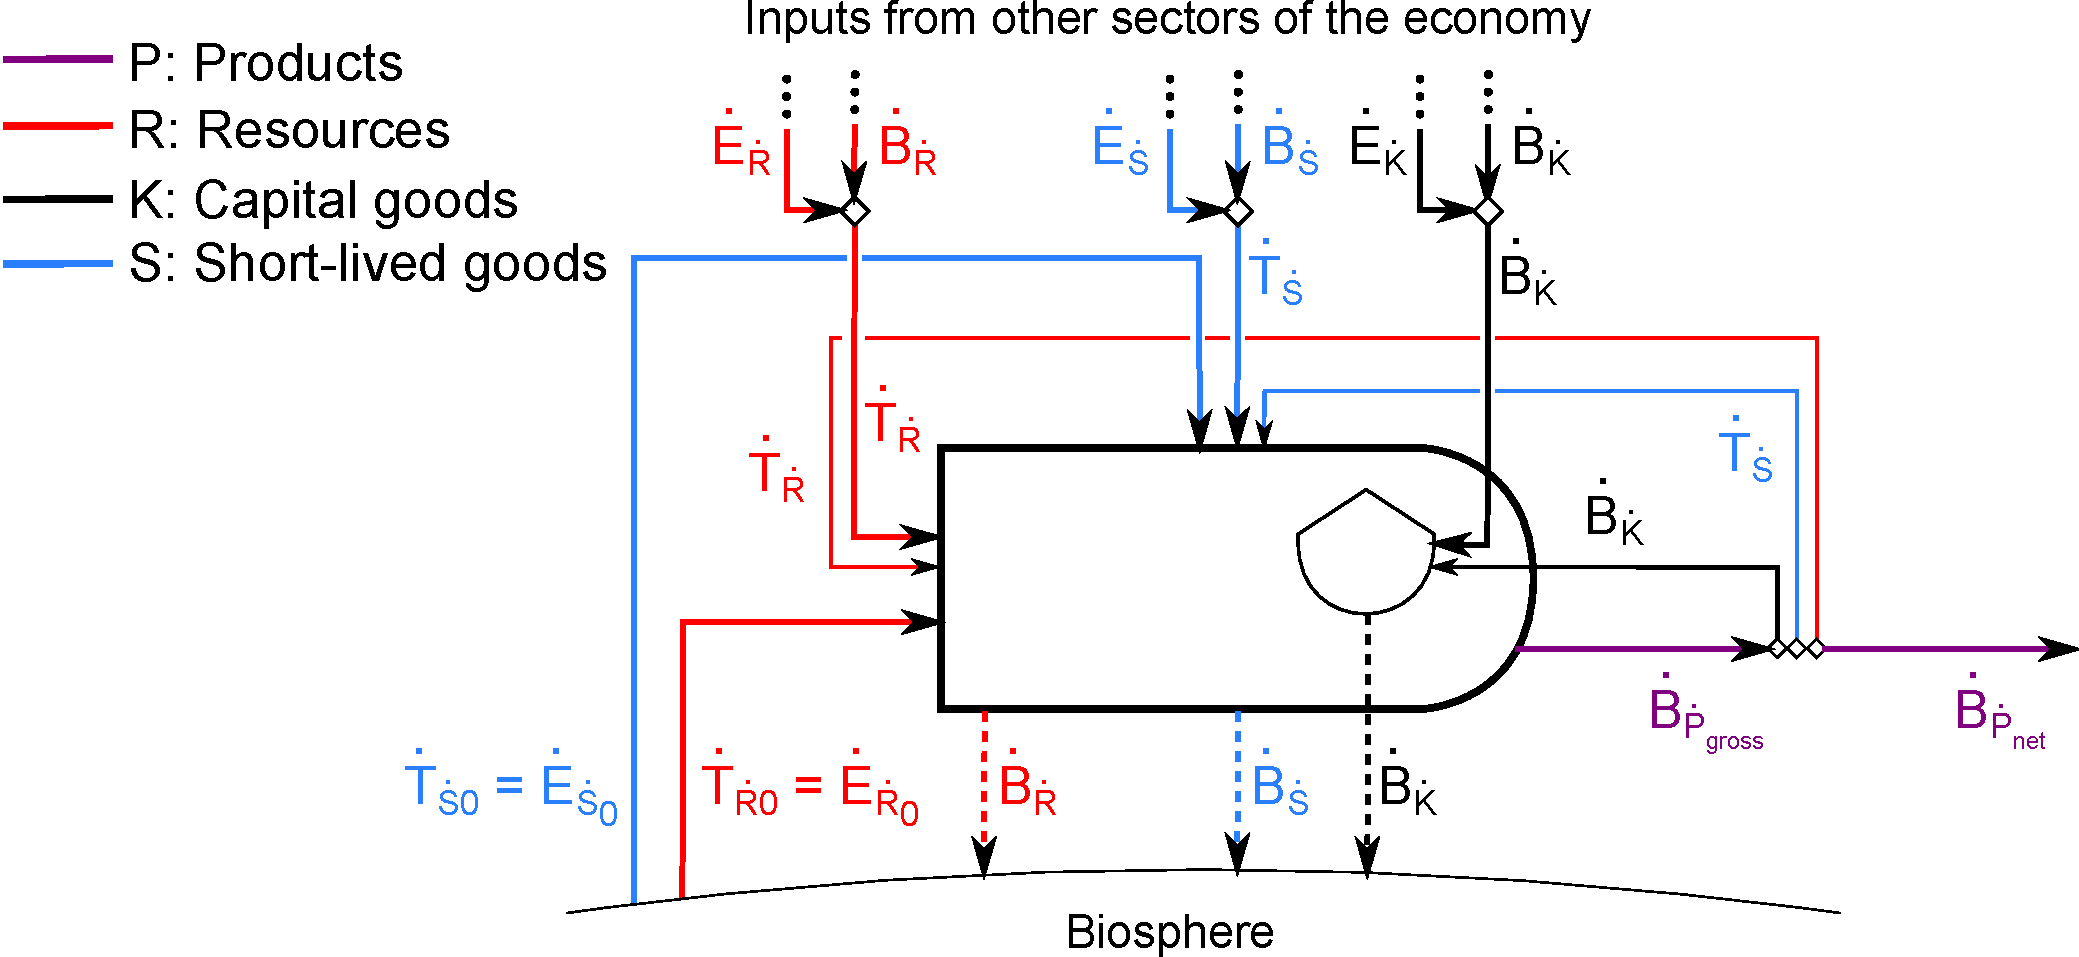
\includegraphics[width=.9\textwidth]{Part_1/Chapter_Embodied/images/PERKS_basic_unit_embodied_energy_content.pdf}
	\caption[Total energy flows for a single sector]{Total energy flows 
	($\dot{T}$) for a single sector of an economy. 
	For the sake of clarity, 
	direct ($\dot{E}$) and embodied ($\dot{B}$) energy flows
	are shown separately for material inflows from other sectors only.
%	**** I think the red $\dot{B}_{\dot{S}}$ and $\dot{E}_{\dot{S}}$
%	should be changed to $\dot{B}_{\dot{R}}$ and $\dot{E}_{\dot{R}}$. MKH **** MCD - well spotted, Sir! ****
}
\label{fig:embodied_single_producer}
\end{figure}

In some cases, a material flow may include 
either direct energy ($\dot{E}$) 
or embodied energy ($\dot{B}$), exclusive. 
For example, the flow of extracted crude oil from the earth 
consists of direct energy only ($\dot{B} = 0$ and $\dot{T} = \dot{E}$), 
because, in this method, no embodied energy ($B$) is added 
to the crude oil until it reaches the downstream side of the oil rig.
The material produced by a non-energy sector of the economy 
consists of indirect energy only ($\dot{E} \approx 0$, 
and therefore $\dot{T} \approx \dot{B}$), 
because direct energy ($E$) produced by 
a non-energy sector is negligible in this economy. 

In other cases, a material flow may include both direct energy flow
($\dot{E}$) \emph{and} embodied energy flow ($\dot{B}$) components.
For example, the outgoing flow of refined petroleum from the energy sector 
has both a direct energy ($\dot{E}$, the energy content of the oil product, 
usually represented by chemical potential energy) 
and embodied energy ($\dot{B}$, which accounts for the energy 
consumed in upstream processes 
to extract and refine the crude oil).\footnote{Outputs from 
agricultural sectors will be similar: 
both (a) the direct energy component (comprising chemical potential energy) 
and (b) the embodied energy component (representing upstream
energy consumed in food production) will be non-zero.}

Most of the I-O literature~\cite{Bullard1975, Herendeen1978} 
applies the following (and often unstated) assumptions:

\begin{enumerate}
	\item flows of total energy ($\dot{T}$) are 
	\emph{conserved},\footnote{Total energy 
	can be neither created nor destroyed.}

	\item steady state conditions exist 
	(i.e., total energy does not accumulate in economic 
	sectors),\footnote{We will see later how the
	steady-state assumption in the literature 
	can introduce errors into I-O analyses.} and
	
	\item the sum of the signed 
	(input is positive, output is negative) 
	total energy inflows of a sector
	is assigned to the products of the sector (i.e., 
	there is no ``waste'' of total energy).
\end{enumerate}

Like the I-O literature, we assume that total energy is conserved
and never wasted.\footnote{Of course, waste heat exists and is
accounted by the First Law of Thermodynamics. However,
waste heat is ignored when accounting for total energy.}
However, we depart from the I-O literature to allow durability of goods 
as represented by total energy accumulation in economic sectors. 
Steady state, this approach is not. 

Total energy ($T$) may accumulate within an economic sector 
as stocks of direct energy materials 
(piles of coal or tanks of oil) 
but also as energy embodied in stocks of capital goods 
(e.g., machinery or buildings). 
The rate of accumulation of total energy 
in a sector of the economy, the biosphere, 
or society is given by the time derivative of total energy:

\begin{equation} \label{eq:T_accum_def}
	\frac{\mathrm{d}T}{\mathrm{d}t} 
	= \frac{\mathrm{d}E}{\mathrm{d}t} 
	+ \frac{\mathrm{d}B}{\mathrm{d}t}.
\end{equation}

The following equation provides a total energy accounting 
for a sector of the economy, where the $\dot{T}$ terms
are signed: positive for total energy input and negative
for total energy output.

\begin{equation} \label{eq:total_energy_accounting}
		\frac{\mathrm{d}T}{\mathrm{d}t}
		= \sum \dot{T}
\end{equation}

By substituting Equations~\ref{eq:T_dot_def} and
\ref{eq:T_accum_def} into 
Equation~\ref{eq:total_energy_accounting},
we obtain

\begin{equation} \label{eq:total_energy_accounting_details}
	\frac{\mathrm{d}E}{\mathrm{d}t} 
	+ \frac{\mathrm{d}B}{\mathrm{d}t}
	= \sum{\left( \dot{E} 
			+ \dot{B} \right)}.
\end{equation}


%+++++++++ Embodied Energy: Embodied Energy Accounting ++++++++++
\subsection{Embodied energy accounting}
%+++++++++

We note that the definition of total energy 
(Equation~\ref{eq:T_def}) includes direct energy ($E$) 
and embodied energy ($B$) terms. 
On the other hand, the First Law of Thermodynamics 
(Equation~\ref{eq:First_Law_with_accumulation})
includes direct energy ($E$) and waste heat ($Q$) terms. 
The consequence of the foregoing difference is that 
an interesting relationship exists between embodied energy ($B$) 
and waste heat ($Q$), as we shall see below. 

To derive an accounting equation for embodied energy, we substitute the 
First Law of Thermodynamics (Equation~\ref{eq:First_Law_with_accumulation})
into the total energy accounting equation (Equation~\ref{eq:total_energy_accounting_details}).

\begin{equation} \label{eq:embodied_energy_accounting}
	\frac{\mathrm{d}B}{\mathrm{d}t}
	= \sum \dot{B} 
	+ \sum \dot{Q}_{out}
\end{equation}

The waste energy terms ($\dot{Q}_{out}$) 
in Equation~\ref{eq:embodied_energy_accounting}
are \emph{outflows} of energy from the sector. 
The embodied energy 
terms ($\dot{B}$) represent embodied energy of inflows
and outflows of material. Splitting the $\dot{B}$ term
into inflows and outflows and rearranging gives

\begin{equation} \label{eq:embodied_energy_accounting_2}
	\frac{\mathrm{d}B}{\mathrm{d}t}
	= \sum \dot{B}_{in}
	- \sum \dot{B}_{out} 
	+ \sum \dot{Q}_{out}
\end{equation}

In words, the rate of accumulation of embodied energy 
in a sector of the economy 
$\left( \frac{\mathrm{d}B}{\mathrm{d}t} \right)$ 
is equal to the sum of the rates of 
inflow of embodied energy into the sector 
	($\dot{B}_{in}$) 
less the rate of output of embodied energy from the sector 
	($\dot{B}_{out}$) 
\emph{plus} the rate of waste direct energy from the sector 
	($\dot{Q}_{out}$). 
The first two terms on the right side of
Equation~\ref{eq:embodied_energy_accounting_2} are expected: 
accumulation is the difference between inflow and outflow rates. 

Rearranging Equation~\ref{eq:embodied_energy_accounting_2}
yields another version of the embodied energy accounting equation:
one that illuminates issues related to 
stages of growth for an economic sector.

\begin{equation} \label{eq:embodied_energy_accounting_3}
	\frac{\mathrm{d}B}{\mathrm{d}t} 
	+ \sum \dot{B}_{out}
	= \sum \dot{B}_{in}
	+ \sum \dot{Q}_{out}
\end{equation}

\noindent From Equation~\ref{eq:embodied_energy_accounting_3},
we see that incoming embodied energy ($\dot{B}_{in}$) and 
waste heat\footnote{Because we have substituted 
the First Law of Thermodynamics into the total energy accounting equation,
$\dot{Q}_{out}$ becomes a proxy for direct energy consumption by the sector.} 
($\dot{Q}_{out}$) can be used to increase either (a)
the embodied energy within a sector of the economy 
$\left( \frac{\mathrm{d}B}{\mathrm{d}t}  \right)$
or (b) the embodied energy output of a sector of the economy 
($\dot{B}_{out}$), 
depending on decisions by actors 
(firms, households, or the government) 
within the sector. 
If the sector is ``building up'' production capacity, 
much of the incoming embodied energy ($\dot{B}_{in}$)
and direct energy consumption (represented by $\dot{Q}_{out}$)
will be used to increase infrastructure 
(and associated embodied energy, $B$) within the sector, 
and $\frac{\mathrm{d}B}{\mathrm{d}t}$ will be positive.
If, on the other hand, the sector is mature, 
much of the incoming embodied energy ($\dot{B}_{in}$)
and direct energy consumption (represented by $\dot{Q}_{out}$)
will be used for production of goods ($\dot{B}_{out}$).
$\frac{\mathrm{d}B}{\mathrm{d}t}$ will be close to zero.
Equation~\ref{eq:embodied_energy_accounting_2} shows that
an economic sector in decline may experience an outflow 
of embodied energy (via products or depreciation\index{depreciation})
in excess of the sum of 
its embodied energy inflows ($\dot{B}_{in}$)
and direct energy consumption (represented by $\dot{Q}_{out}$),
and $\frac{\mathrm{d}B}{\mathrm{d}t}$ will be negative.

Equations~\ref{eq:embodied_energy_accounting_2}
and~\ref{eq:embodied_energy_accounting_3} 
highlight a contrast between 
the present dynamic analysis and the I-O literature.
The traditional assumption of steady-state conditions 
in economic sectors is tantamount to assuming that
$\frac{\mathrm{d}B}{\mathrm{d}t} = 0$ in 
Equations~\ref{eq:embodied_energy_accounting_2}
and~\ref{eq:embodied_energy_accounting_3}.
That assumption precludes analysis of stages of growth 
and the embodied energy implications thereof.

Equations~\ref{eq:embodied_energy_accounting_2}
and~\ref{eq:embodied_energy_accounting_3} 
are generalized embodied energy accounting equations that we will
see again for Examples~A-C in the sections that follow.


%%%%%%%%%% Embodied Energy: Example A %%%%%%%%%%
\section{Example A: single-sector economy} % chktex 13
%%%%%%%%%%

Figure~\ref{fig:A_total_energy_T_dot} shows the flows 
of total energy ($\dot{T}$) through the single-sector economy.

\begin{figure}[!ht]
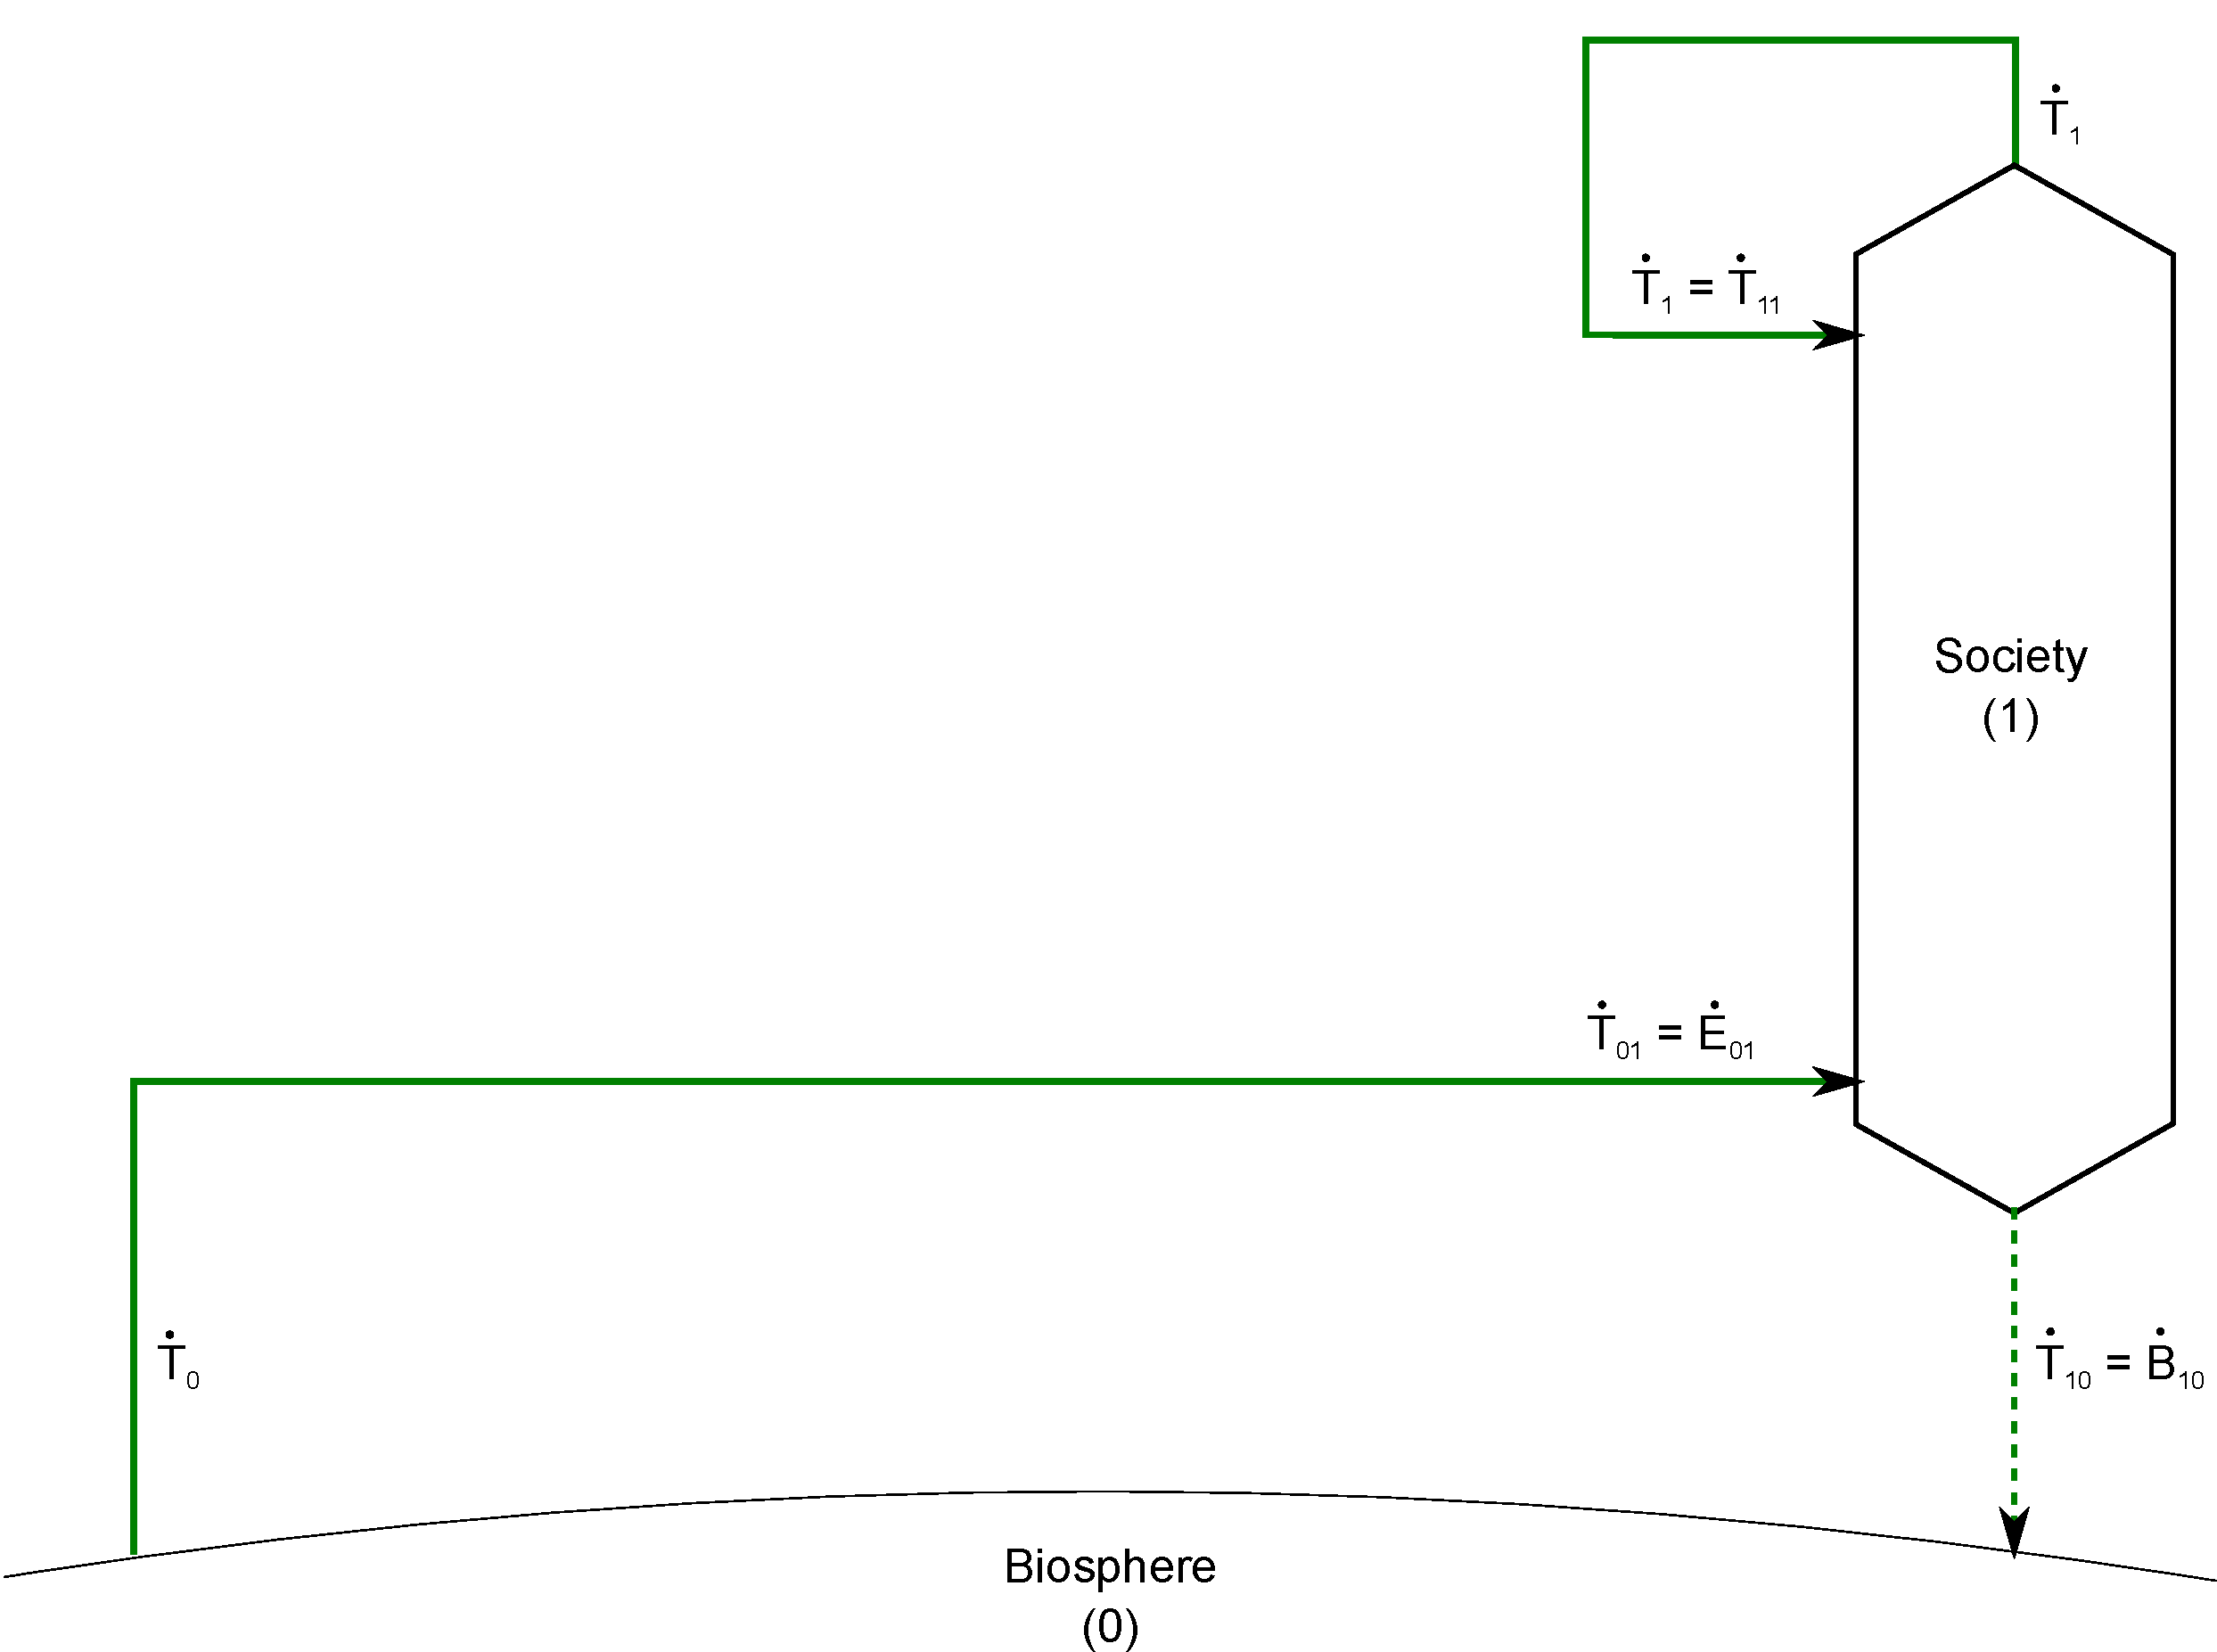
\includegraphics[width=1.0\linewidth]{Part_1/Chapter_Embodied/images/1_sector_embodied_energy.pdf}
\caption[Total energy flows in a one-sector economy]{Total energy flows ($\dot{T}$) in a one-sector economy.}
\label{fig:A_total_energy_T_dot}
\end{figure}

As discussed above, we follow the I-O literature in assuming that 
total energy ($T$) is conserved. 
A total energy accounting around the biosphere (0)
and the single-sector economy (1) gives

\begin{equation} \label{eq:A_T_acct_0}
	\frac{\mathrm{d}T_{0}}{\mathrm{d}t} 
	= \dot{T}_{10} 
	- \dot{T}_{01},
\end{equation}

\noindent and

\begin{equation} \label{eq:A_T_acct_1}
	\frac{\mathrm{d}T_{1}}{\mathrm{d}t} 
	= \dot{T}_{01} 
	+ \dot{T}_{11}
	- \dot{T}_{1}
	- \dot{T}_{10}.
\end{equation}

Substituting Equations~\ref{eq:T_dot_def} and
\ref{eq:T_accum_def} into 
Equations~\ref{eq:A_T_acct_0} and~\ref{eq:A_T_acct_1}
yields

\begin{equation} \label{eq:A_total_energy_0}
	\frac{\mathrm{d}E_{0}}{\mathrm{d}t} 
	+ \frac{\mathrm{d}B_{0}}{\mathrm{d}t} 
	= \dot{E}_{10} 
	+ \dot{B}_{10} 
	- \dot{E}_{01}
	- \dot{B}_{01}
\end{equation}

\noindent and

\begin{equation} \label{eq:A_total_energy_1}
	\frac{\mathrm{d}E_{1}}{\mathrm{d}t} 
	+ \frac{\mathrm{d}B_{1}}{\mathrm{d}t} 
	= \dot{E}_{01} 
	+ \dot{B}_{01} 
	+ \dot{E}_{11}
	+ \dot{B}_{11}
	- \dot{E}_{1}
	- \dot{B}_{1}
	- \dot{E}_{10}
	- \dot{B}_{10}.	
\end{equation}

At this point, we can proceed in two directions.
The first direction, 
simplifying Equations~\ref{eq:A_total_energy_0} 
and~\ref{eq:A_total_energy_1}, 
provides an intuitive result. 
The second direction,
substituting the First Law of Thermodynamics into 
Equations~\ref{eq:A_total_energy_0} 
and~\ref{eq:A_total_energy_1}, 
provides the advantage of cancelling most of the direct energy terms.
We begin with the first approach: simplification.


%+++++++++ Simplified embodied energy ++++++++++
\subsection{Simplification of the embodied energy accounting equation} % (fold)
\label{sec:A_simplified_embodied}
%+++++++++

To simplify Equations~\ref{eq:A_total_energy_0} 
and~\ref{eq:A_total_energy_1},
we first realize that, by definition, no embodied energy flows from 
the earth with extracted material, so $\dot{B}_{01} = 0$
and $\dot{T}_{0} = \dot{E}_{01}$ as shown in Figure~\ref{fig:A_total_energy_T_dot}.
Second, we can assume that direct energy ($E$) does not accumulate
in the economy such that 
$\frac{\mathrm{d}E_0}{\mathrm{d}t} = 0$ and
$\frac{\mathrm{d}E_1}{\mathrm{d}t} = 0$.
Finally, we note that $\dot{E}_{10} = 0$, 
because society does not supply direct energy 
to the biosphere. Thus, Equations~\ref{eq:A_total_energy_0}
and~\ref{eq:A_total_energy_1} become

\begin{equation} \label{eq:A_total_energy_0_simp}
	\frac{\mathrm{d}B_{0}}{\mathrm{d}t} 
	= \dot{B}_{10} 
	- \dot{E}_{01}
\end{equation}

\noindent and

\begin{equation} \label{eq:A_total_energy_1_simp}
	\frac{\mathrm{d}B_{1}}{\mathrm{d}t} 
	= \dot{E}_{01} 
	+ \dot{E}_{11}
	+ \dot{B}_{11}
	- \dot{E}_{1}
	- \dot{B}_{1}
	- \dot{B}_{10}.	
\end{equation}

These equations show that direct energy consumed by a 
sector ($\dot{E}_{01}$) increases the energy embodied within the sector ($B_1$), 
whereas the waste from the sector produces an embodied
energy outflow ($\dot{B}_{10}$) that reduces 
the energy embodied within the sector. 


%+++++++++ First Law embodied energy ++++++++++
\subsection{Substitution of First Law into the embodied energy accounting equation} % (fold)
\label{subsec:A_first_law_embodied}
%+++++++++

The second approach to the derivation of embodied energy
accounting equations is to substitute the First Law
(Equations~\ref{eq:dE_0/dt_single_sector} and~\ref{eq:dE_1/dt_single_sector}) 
into the total energy accounting equations 
(Equations~\ref{eq:A_total_energy_0} and~\ref{eq:A_total_energy_1}). 
\begin{equation} \label{eq:A_dB0/dt}
	\frac{\mathrm{d}B_{0}}{\mathrm{d}t} 
	= \dot{E}_{10}
	+ \dot{B}_{10} 
	- \dot{B}_{01}
	- \dot{Q}_{10}
\end{equation}

\begin{equation} \label{eq:A_dB1/dt}
	\frac{\mathrm{d}B_{1}}{\mathrm{d}t} 
	= \dot{B}_{01} 
	+ \dot{B}_{11}
	- \dot{B}_{1}
	- \dot{B}_{10}
	- \dot{E}_{10}
	+ \dot{Q}_{10}
\end{equation}

This substitution has the advantage of canceling most 
of the direct energy terms from the embodied energy accounting equations.
And, it is no longer necessary to assume that the 
accumulation rate of direct energy 
$\left( \frac{\mathrm{d}E}{\mathrm{d}t} \right)$
is zero, because the 
$\frac{\mathrm{d}E}{\mathrm{d}t}$
term is cancelled by the substitution.

Note that the Equation~\ref{eq:A_dB0/dt} includes the
term $-\dot{Q}_{10}$, which, at first glance,
appears different from 
Equation~\ref{eq:embodied_energy_accounting_2}.\footnote{Equation~\ref{eq:embodied_energy_accounting_2}
has a positive sign for the waste energy term (+ $\dot{Q}_{out}$),
whereas Equation~\ref{eq:A_dB0/dt} has a 
negative sign for the waste energy term ($- \dot{Q}_{10}$).}
However, upon realizing that $\dot{Q}_{10}$ is an \emph{inflow}
of waste energy into the biosphere, we can use $\dot{Q}_{10} = - \dot{Q}_{01}$
to rewrite Equation~\ref{eq:A_dB0/dt} with an \emph{outflow} 
term,

\begin{equation} \label{eq:A_dB0/dt_waste_outflow}
	\frac{\mathrm{d}B_{0}}{\mathrm{d}t} 
	= \dot{E}_{10}
	+ \dot{B}_{10} 
	- \dot{B}_{01}
	+ \dot{Q}_{01},
\end{equation}

\noindent thereby maintining consistency with
Equation~\ref{eq:embodied_energy_accounting_2}.

We can simplify 
Equations~\ref{eq:A_dB0/dt} and~\ref{eq:A_dB1/dt} 
using the assumptions of Section~\ref{sec:A_simplified_embodied} 
(namely, that $\dot{B}_{01} = 0$ and $\dot{E}_{10} = 0$)
to obtain

\begin{equation} \label{eq:A_dB0/dt_simp}
	\frac{\mathrm{d}B_{0}}{\mathrm{d}t} 
	= \dot{B}_{10} 
	- \dot{Q}_{10}
\end{equation}

\noindent and

\begin{equation} \label{eq:A_dB1/dt_simp_prelim}
	\frac{\mathrm{d}B_{1}}{\mathrm{d}t} 
	= \dot{B}_{11}
	- \dot{B}_{1}
	- \dot{B}_{10}
	+ \dot{Q}_{10}.
\end{equation}

\noindent{}The material model of this framework (see Chapter~\ref{chap:materials})
indicates that materials are comprised of 
resources ($R$), 
short-lived materials ($S$), and
capital ($K$).
Thus, we can write 

\begin{equation}
	\frac{\mathrm{d}B_{1}}{\mathrm{d}t} 
	= \frac{\mathrm{d}B_{R,1}}{\mathrm{d}t} 
	+ \frac{\mathrm{d}B_{S,1}}{\mathrm{d}t} 
	+ \frac{\mathrm{d}B_{K,1}}{\mathrm{d}t},
\end{equation}

\noindent{}but neither resources ($R$) nor short-lived
materials ($S$) accumulate in economic sectors at a significant rate.
Thus, 

\begin{equation} \label{eq:A-dBdt_simplification}
	\frac{\mathrm{d}B_{1}}{\mathrm{d}t} 
	= \frac{\mathrm{d}B_{K_{1}}}{\mathrm{d}t}.
\end{equation}

\noindent{}We can substitute Equation~\ref{eq:A-dBdt_simplification}
into Equation~\ref{eq:A_dB1/dt_simp_prelim} to obtain

\begin{equation} \label{eq:A_dB1/dt_simp}
	\frac{\mathrm{d}B_{K,1}}{\mathrm{d}t}
	= \dot{B}_{11}
	- \dot{B}_{1}
	- \dot{B}_{10}
	+ \dot{Q}_{10}.
\end{equation}

\noindent{}Equations~\ref{eq:A_dB0/dt_simp} and~\ref{eq:A_dB1/dt_simp} are 
the embodied energy accounting equations for Example~A.

In Examples~B and C following, we will choose the approach of 
this section, namely substitution of the 
First Law of Thermodynamics into the total energy accounting equation
(instead of simplifying the total energy equation 
as discussed in Section~\ref{sec:A_simplified_embodied}),
because of the benefit of canceling direct energy flow terms ($\dot{E}$). 


%+++++++++ Depreciation ++++++++++
\subsection{Physical depreciation}\index{depreciation}
\label{sec:depreciation_embodied}
%+++++++++

The term $\dot{B}_{10}$ in Equation~\ref{eq:A_dB1/dt_simp}
represents the disposal rate 
of embodied energy from Society (1) to the Biosphere (0). 
Figure~\ref{fig:A_materials} shows that the outgoing material flow
from Society (1) is comprised of 
resources ($\dot{R}_{10}$),
short-lived materials ($\dot{S}_{10}$), and 
capital ($\dot{K}_{10}$). 
Each of these material flows will have associated embodied energy such that

\begin{equation} \label{eq:A-depreciation-of-B}
	\dot{B}_{10}
	= \dot{B}_{\dot{R}_{10}}
	+ \dot{B}_{\dot{S}_{10}}
	+ \dot{B}_{\dot{K}_{10}}.
\end{equation}

The term $\dot{B}_{\dot{K}_{10}}$ represents the energy embodied
in depreciated phyiscal assets.
Physical depreciation\index{depreciation!physical} 
is counted at the moment when material physically departs an economic sector 
and enters the biosphere, presumably a landfill, 
where the material in the wasted assets will decay.
Financial depreciation\index{depreciation!financial}
is usually faster than physical depreciation
according to rates set by accounting rules.
The embodied energy associated with physical depreciation ($\dot{B}_{\dot{K}_{10}}$)
can be represented by a depreciation term such as

\begin{equation} \label{eq:depreciation_term_defined}
	\dot{B}_{\dot{K}_{10}} 
	= \gamma_{B,1} B_{K_{1}},
\end{equation}

\noindent{}where $\gamma_{B}$ represents the depreciation rate 
of embodied energy in units of inverse time (e.g., 1/year) 
with $\gamma_{B} > 0$.\footnote{Note that $\gamma_B$ will, in general,
be different from $\gamma_{K}$ defined in Section~\ref{sec:A_materials}.
$\gamma_{B}$ will equal $\gamma_{K}$ if and only if 
the depreciated capital has an embodied energy content that is 
identical to the average embodied energy content 
of the sector on a per-unit-mass basis.}
The depreciation rate ($\gamma_{B}$) indicates that 
a fraction of the energy embodied in capital stock
is disposed over a period of time (e.g., $\gamma_{B} = 0.05$/year). 
In the absence of other inputs or outputs, 
this depreciation function provides exponential decay 
of embodied energy ($B$) in an economic sector. 
$\gamma_{B}$ is, in general, a function of time.

Equation~\ref{eq:depreciation_term_defined} can be substituted into
Equation~\ref{eq:A-depreciation-of-B} to obtain

\begin{equation} \label{eq:B_10_term}
	\dot{B}_{10}
	= \dot{B}_{\dot{R}_{10}}
	+ \dot{B}_{\dot{S}_{10}}
	+ \gamma_{B,1} B_{K_{1}}.	
\end{equation}

\noindent{}Equation~\ref{eq:B_10_term} 
can be substituted into Equations~\ref{eq:A_dB0/dt_simp}
and~\ref{eq:A_dB1/dt_simp} to obtain 

\begin{equation} \label{eq:A-dB0/dt_with_depreciation_gamma}
	\frac{\mathrm{d}B_{0}}{\mathrm{d}t} 
	= \dot{B}_{\dot{R}_{10}}
	+ \dot{B}_{\dot{S}_{10}}
	+ \gamma_{B,1} B_{K_{1}}
	- \dot{Q}_{10} 
\end{equation}

\noindent{}and

\begin{equation} \label{eq:A-dB1/dt_with_depreciation_gamma}
	\frac{\mathrm{d}B_{K_{1}}}{\mathrm{d}t} 
	= \dot{B}_{11}
	- \dot{B}_{1}
	- \dot{B}_{\dot{R}_{10}}
	- \dot{B}_{\dot{S}_{10}}
	- \gamma_{B,1} B_{K_{1}}
	+ \dot{Q}_{10}.
\end{equation}

\noindent{}Equation~\ref{eq:A-dB1/dt_with_depreciation_gamma} 
indicates that the accumulation rate 
of embodied energy in an economic sector 
$\left( \frac{\mathrm{d}B_{K_{1}}}{\mathrm{d}t} \right)$
is equal to the sum of the embodied energy input to the sector~($\dot{B}_{11}$)
and waste heat from the economic sector~($\dot{Q}_{10}$),
less embodied energy the leaves the sector in its products~($\dot{B}_{1}$), 
less the rate of disposal of embodied energy associated with 
scrap resources~($\dot{B}_{\dot{R}_{10}}$),
short-lived material~($\dot{B}_{\dot{S}_{10}}$), and
depreciated capital stock~($\gamma_{B,1} B_{K_{1}}$).

We turn now to Example~B, a two-sector economy.


%%%%%%%%%% Embodied Energy: Example B %%%%%%%%%%
\section{Example B: two-sector economy} % chktex 13
\label{sec:Embodied_Energy_Example_B}
%%%%%%%%%%

For the two-sector economy of Figures~\ref{fig:B_materials}
and~\ref{fig:B_energy}, we again follow the I-O literature 
by assuming that total energy ($T$) is conserved. 
Figure~\ref{fig:B_total_energy} shows total energy
flows for the two-sector economy.

\begin{figure}[!ht]
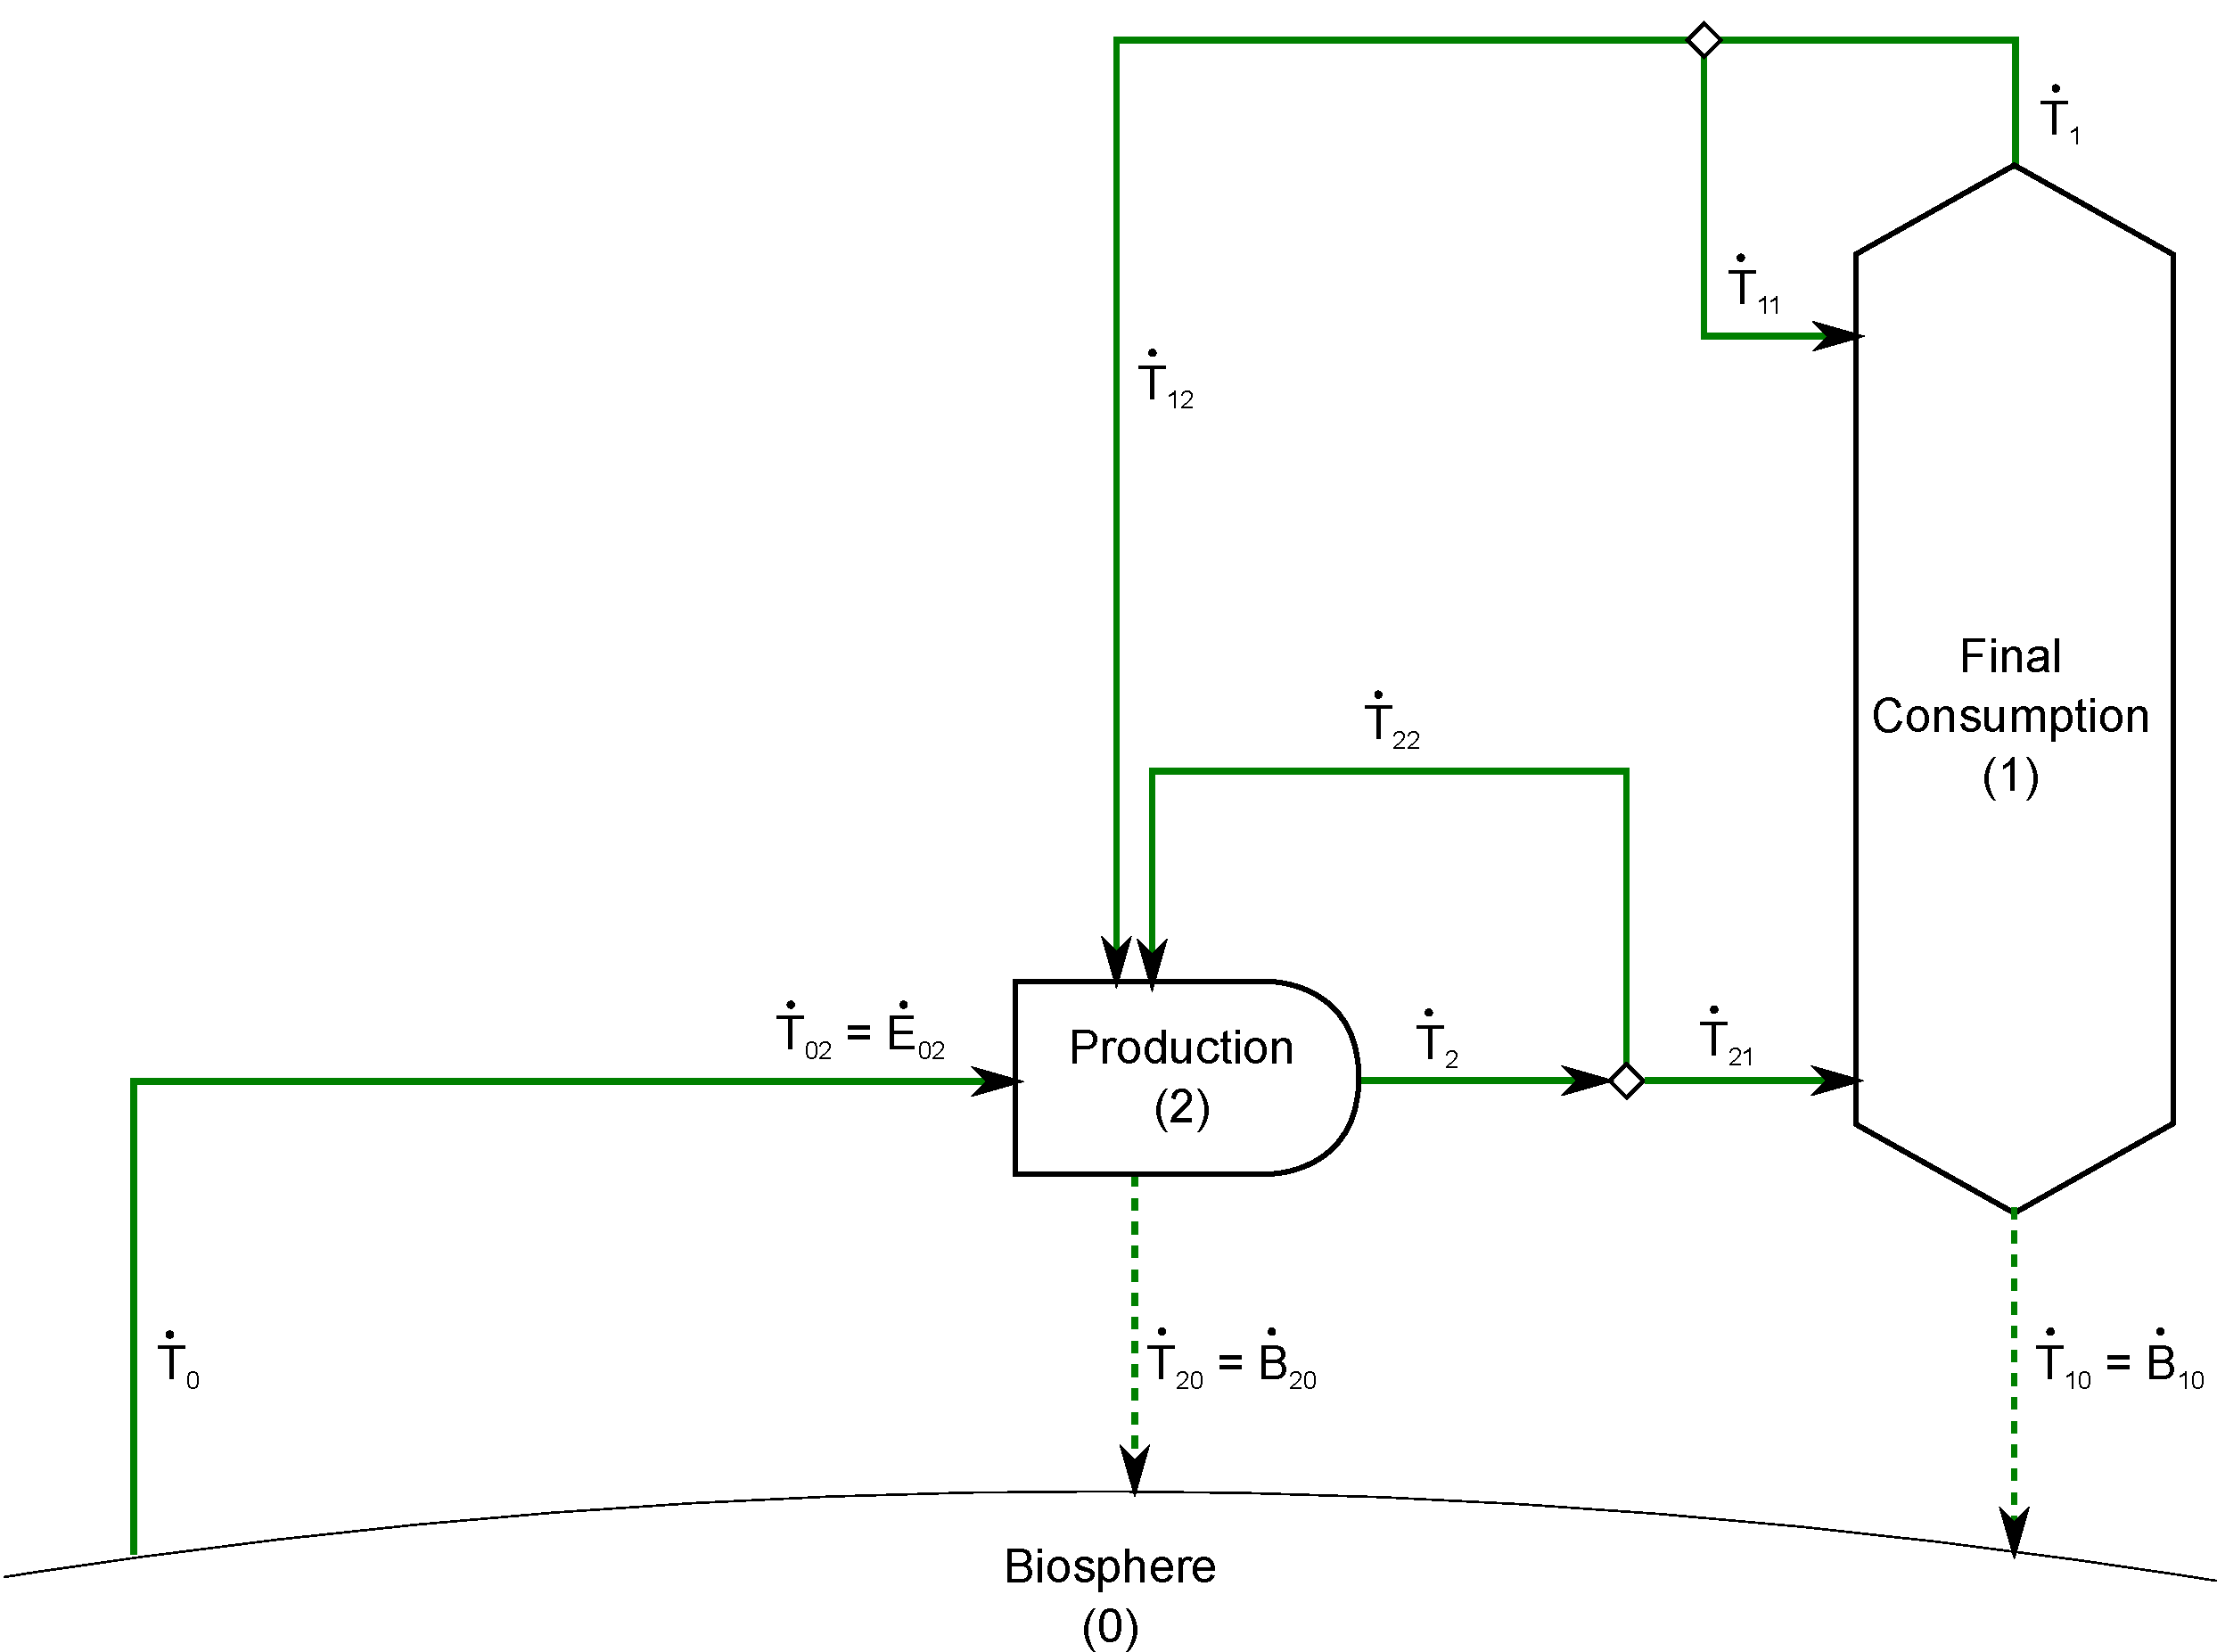
\includegraphics[width=0.9\linewidth]{Part_1/Chapter_Embodied/images/2_sector_embodied_energy.pdf}
\caption[Flows of total energy in a two-sector economy.]{Flows of total energy ($\dot{T}$) in a two-sector economy.}
\label{fig:B_total_energy}
\end{figure}

Accounting for accumulation of total energy and using the assumption 
that total energy is conserved, we can write the following equations.

\begin{equation} \label{eq:CV_T_0}
	\frac{\mathrm{d}T_{0}}{\mathrm{d}t} 	 
	= \dot{T}_{10} 
	+ \dot{T}_{20} 
	- \dot{T}_{02},
\end{equation}

\begin{equation} \label{eq:CV_T_1}
	\frac{\mathrm{d}T_{1}}{\mathrm{d}t} 	 
	= \dot{T}_{11}
	+ \dot{T}_{21} 
	- \dot{T}_{1}
	- \dot{T}_{10},
\end{equation}

\noindent and

\begin{equation} \label{eq:CV_T_2}
	\frac{\mathrm{d}T_{2}}{\mathrm{d}t} 	 
	= \dot{T}_{02} 
	+ \dot{T}_{12}
	+ \dot{T}_{22} 
	- \dot{T}_{2} 
	- \dot{T}_{20}.
\end{equation}

Substituting Equations~\ref{eq:T_dot_def} 
and~\ref{eq:T_accum_def} into 
Equations~\ref{eq:CV_T_0} through
\ref{eq:CV_T_2} gives

\begin{equation} \label{eq:CV_dB_0}
	\frac{\mathrm{d}B_{0}}{\mathrm{d}t} 
	+ \frac{\mathrm{d}E_{0}}{\mathrm{d}t} 
	= \dot{E}_{10} 
	+ \dot{B}_{10} 
	+ \dot{E}_{20} 
	+ \dot{B}_{20} 
	- \dot{E}_{02} 
	- \dot{B}_{02},
\end{equation}

\begin{equation} \label{eq:CV_dB_1}
	\frac{\mathrm{d}B_{1}}{\mathrm{d}t} 
	+ \frac{\mathrm{d}E_{1}}{\mathrm{d}t} 
	= \dot{E}_{11}
	+ \dot{B}_{11}
	+ \dot{E}_{21} 
	+ \dot{B}_{21} 
	- \dot{E}_1
	- \dot{B}_1
	- \dot{E}_{10} 
	- \dot{B}_{10},
\end{equation}

\noindent and 

\begin{equation} \label{eq:CV_dB_2}
	\frac{\mathrm{d}B_{2}}{\mathrm{d}t} 
	+ \frac{\mathrm{d}E_{2}}{\mathrm{d}t} 
	= \dot{E}_{02} 
	+ \dot{B}_{02} 
	+ \dot{E}_{12}
	+ \dot{B}_{12}
	+ \dot{E}_{22} 
	+ \dot{B}_{22} 
	- \dot{E}_{2} 
	- \dot{B}_{2} 
	- \dot{E}_{20} 
	- \dot{B}_{20}.
\end{equation}

As in Example~A, we can substitute the First Law of Thermodynamics 
(Equations~\ref{eq:CV_E_dot_0}--\ref{eq:CV_E_dot_2})
into the total energy accounting equations
(Equations~\ref{eq:CV_dB_0}--\ref{eq:CV_dB_2}) 
and employ the assumptions that 
$\dot{E}_{i0} = 0$ and
$\dot{B}_{0j} = 0$ 
to obtain

\begin{equation} \label{eq:B_embodied_energy_accounting_0}
	\frac{\mathrm{d}B_{0}}{\mathrm{d}t} 
	= \dot{B}_{10} 
	+ \dot{B}_{20} 
	- \dot{Q}_{10} 
	- \dot{Q}_{20}, 
\end{equation}

\begin{equation} \label{eq:B_embodied_energy_accounting_1}
	\frac{\mathrm{d}B_{1}}{\mathrm{d}t} 
	= \dot{B}_{11} 
	+ \dot{B}_{21}
	- \dot{B}_{2} 
	- \dot{B}_{10}
	+ \dot{Q}_{10},
\end{equation}

\noindent and

\begin{equation} \label{eq:B_embodied_energy_accounting_2}
	\frac{\mathrm{d}B_2}{\mathrm{d}t} 
	= \dot{B}_{12} 
	+ \dot{B}_{22} 
	- \dot{B}_{2}
	- \dot{B}_{20} 
	+ \dot{Q}_{20}.
\end{equation}

Similar to Example~A, we observe that the accumulation rate 
of embodied energy in the economic sectors (1 and 2) 
is the sum of the rates of waste heat flowing from the sector 
($\dot{Q}_{20}$) and embodied energy into the sector 
($\dot{B}_{12} + \dot{B}_{22}$) 
less the rate of embodied energy leaving the sector 
on its output streams ($\dot{B}_{2} + \dot{B}_{20}$).

Equations~\ref{eq:B_embodied_energy_accounting_0}--\ref{eq:B_embodied_energy_accounting_2}
can be simplified using sums:

\begin{equation} \label{eq:B_embodied_energy_accounting_0_sum}
	\frac{\mathrm{d}B_{0}}{\mathrm{d}t} 
	= \sum\limits_{i=1}^n\dot{B}_{i0} 
	- \sum\limits_{i=1}^n\dot{Q}_{i0} 
\end{equation}

\noindent and

\begin{equation} \label{eq:B_embodied_energy_accounting_12_sum}
	\frac{\mathrm{d}B_{j}}{\mathrm{d}t} 
	= \sum\limits_{i=1}^n\dot{B}_{ij} 
	- \dot{B}_{j}
	- \dot{B}_{j0} 
	+ \dot{Q}_{j0},
\end{equation}

\noindent where $j \in [1, n]$.

As in Example~A, 
we can disaggregate the accumulation and waste embodied energy terms 
and express physical waste of capital stock as depreciation 
in Equations~\ref{eq:B_embodied_energy_accounting_0_sum}
and~\ref{eq:B_embodied_energy_accounting_12_sum}
to obtain

\begin{equation} \label{eq:B_embodied_energy_accounting_0_with_depreciation}
	\frac{\mathrm{d}B_{0}}{\mathrm{d}t} 
	= \sum\limits_{i=1}^n 
		\left( \dot{B}_{\dot{R}_{i0}} 
				+ \dot{B}_{\dot{S}_{i0}} 
				+ \gamma_{B,i} B_{K_{i}} \right)
	- \sum\limits_{i=1}^n\dot{Q}_{i0} 
\end{equation}

\noindent and

\begin{equation} \label{eq:B_embodied_energy_accounting_12_with_depreciation}
	\frac{\mathrm{d}B_{K,j}}{\mathrm{d}t} 
	= \sum\limits_{i=1}^n\dot{B}_{ij} 
	- \dot{B}_{j}
	- \left( \dot{B}_{\dot{R}_{j0}}
		+ \dot{B}_{\dot{S}_{j0}}
		+ \gamma_{B,j} B_{K_{j}} \right)
	+ \dot{Q}_{j0}.
\end{equation}

In the next section, we apply embodied energy accounting to 
Example~C, a three-sector economy.


%%%%%%%%%% Embodied Energy: Example C %%%%%%%%%%
\section{Example C: three-sector economy} % chktex 13
\label{sec:Embodied_Energy_Example_C}
%%%%%%%%%%

Again, we begin with the diagram showing total energy ($\dot{T}$) flows
among the economic sectors of Example~C (Figure~\ref{fig:C_total_energy}).

\begin{figure}[!ht]
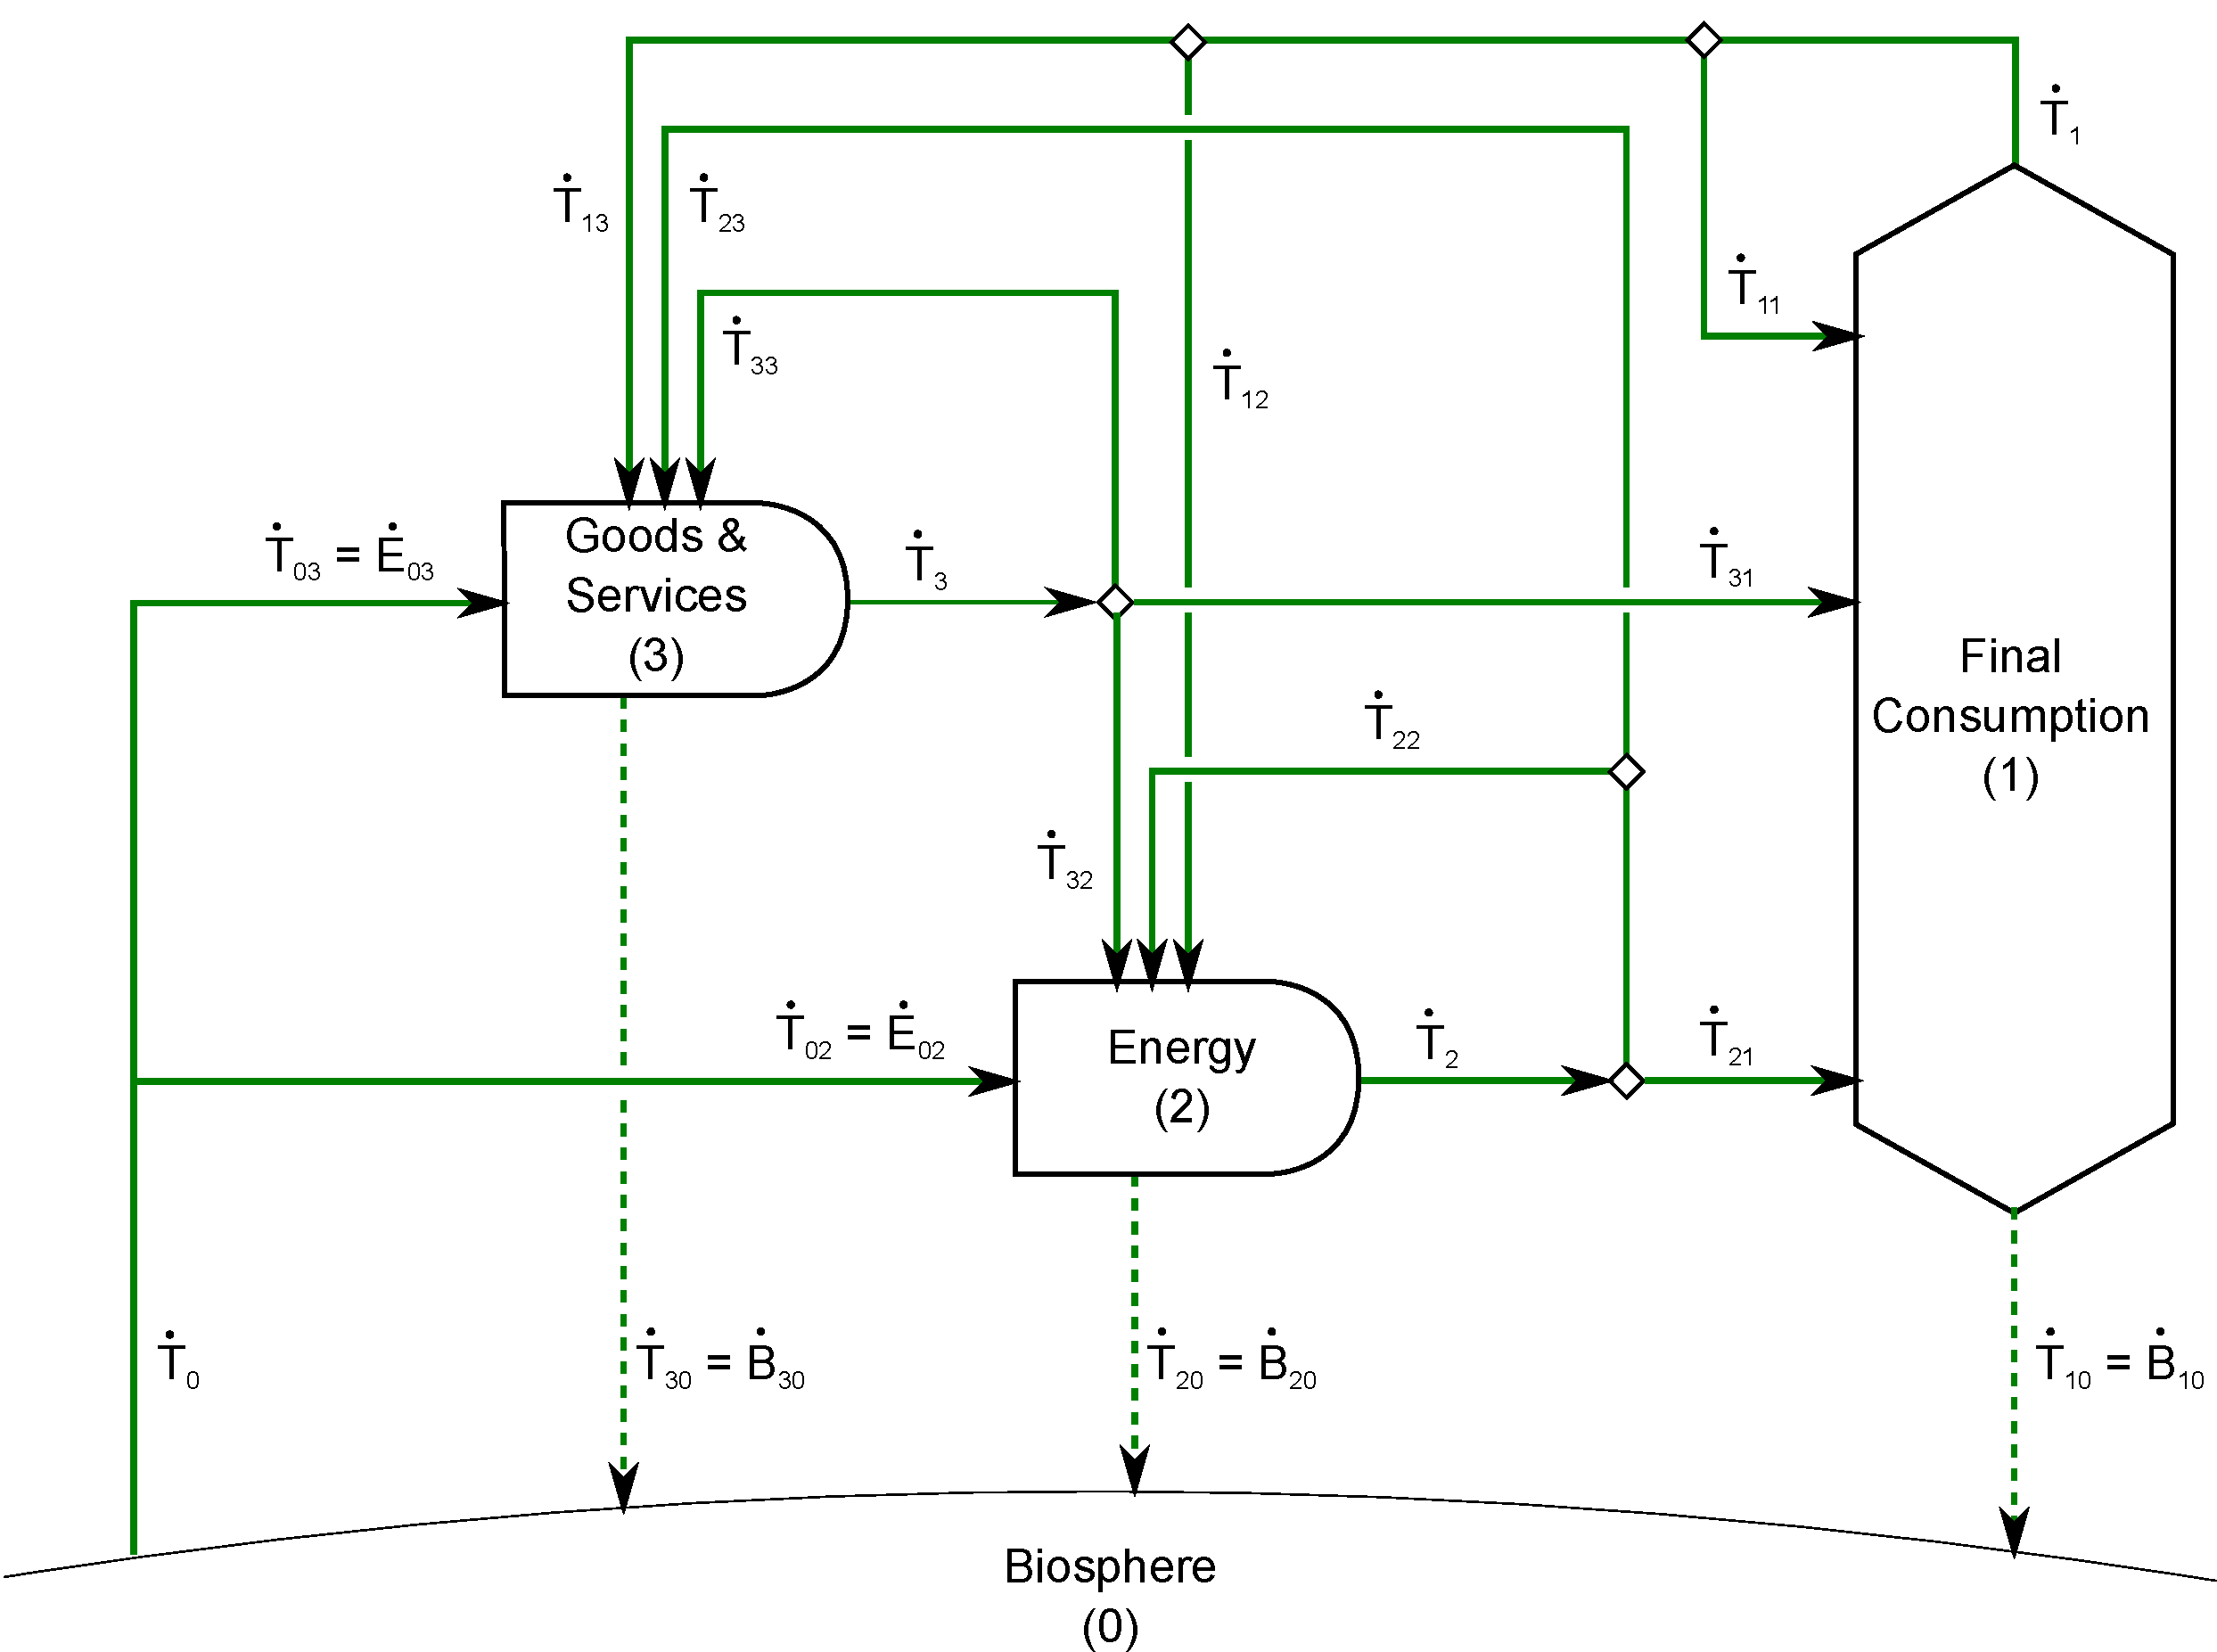
\includegraphics[width=1.0\linewidth]{Part_1/Chapter_Embodied/images/3_sector_embodied_energy.pdf}
\caption[Flows of total energy in a three-sector economy.]{Flows of total energy ($\dot{T}$) in a three-sector economy.}
\label{fig:C_total_energy}
\end{figure}

Accounting for accumulation of total energy and 
applying the assumption that total energy is conserved, 
we can write the following equations.
We build from the derivation in Section~\ref{sec:Embodied_Energy_Example_B}
and utilize sums for each equation below.

\begin{equation} \label{eq:C-CV_T_0}
	\frac{\mathrm{d}T_{0}}{\mathrm{d}t} 	 
	= \sum\limits_{i=1}^{n} \dot{T}_{i0}
	- \sum\limits_{j=1}^{n} \dot{T}_{0j}
\end{equation}

\noindent and

\begin{equation} \label{eq:C-CV_T_123}
	\frac{\mathrm{d}T_{j}}{\mathrm{d}t} 	 
	= \sum\limits_{i=0}^{n} \dot{T}_{ij}
	- \dot{T}_{j}
	- \dot{T}_{j0}.
\end{equation}

\noindent where $j \in [1, n]$.

Substituting Equations~\ref{eq:T_dot_def} 
and~\ref{eq:T_accum_def} into 
Equations~\ref{eq:C-CV_T_0} and
\ref{eq:C-CV_T_123} gives

\begin{equation} \label{eq:C-CV_dB_0}
	\frac{\mathrm{d}E_{0}}{\mathrm{d}t}
	+ \frac{\mathrm{d}B_{0}}{\mathrm{d}t} 	 
	= \sum\limits_{i=1}^{n} \dot{E}_{i0}
	+ \sum\limits_{i=1}^{n} \dot{B}_{i0}
	- \sum\limits_{j=1}^{n} \dot{E}_{0j}
	- \sum\limits_{j=1}^{n} \dot{B}_{0j}
\end{equation}

\noindent and

\begin{equation} \label{eq:C-CV_dB_123}
	\frac{\mathrm{d}E_{j}}{\mathrm{d}t}
	+ \frac{\mathrm{d}B_{j}}{\mathrm{d}t} 	 
	= \sum\limits_{i=0}^{n} \dot{E}_{ij}
	+ \sum\limits_{i=0}^{n} \dot{B}_{ij}
	- \dot{E}_{j}
	- \dot{B}_{j}
	- \dot{E}_{j0}
	- \dot{B}_{j0}.
\end{equation}

Substituting the First Law of Thermodynamics 
(Equations~\ref{eq:C-CV_E_biosphere_general} and~\ref{eq:C-CV_E_econ_general}) 
into the total energy accounting equations 
(Equations~\ref{eq:C-CV_dB_0} and~\ref{eq:C-CV_dB_123}) 
and recognizing that $\dot{B}_{0j} = 0$ for $j \in [1, n]$
and $\dot{E}_{i0} = 0$ for $i \in [1, n]$
gives embodied energy accounting equations for Example~C: % chktex 13

\begin{equation} \label{eq:C-embodied_acct_0}
	\frac{\mathrm{d}B_{0}}{\mathrm{d}t} 	 
	= \sum\limits_{i=1}^{n} \dot{B}_{i0}
	- \sum\limits_{i=1}^{n} \dot{Q}_{i0}
\end{equation}

\begin{equation} \label{eq:C-embodied_acct_123}
	\frac{\mathrm{d}B_{j}}{\mathrm{d}t} 	 
	= \sum\limits_{i=0}^{n} \dot{B}_{ij}
	- \dot{B}_{j}
	- \dot{B}_{j0}
	+ \dot{Q}_{j0} 
\end{equation}

As in Example~B, 
we can disaggregate the accumulation and waste embodied energy terms 
and express physical waste of capital stock as depreciation 
in Equations~\ref{eq:C-embodied_acct_0}
and~\ref{eq:C-embodied_acct_123}
to obtain

\begin{equation} \label{eq:C_embodied_energy_accounting_0_with_depreciation}
	\frac{\mathrm{d}B_{0}}{\mathrm{d}t} 
	= \sum\limits_{i=1}^n 
		\left( \dot{B}_{\dot{R}_{i0}} 
				+ \dot{B}_{\dot{S}_{i0}} 
				+ \gamma_{B,i} B_{K_{i}} \right)
	- \sum\limits_{i=1}^n\dot{Q}_{i0} 
\end{equation}

\noindent and

\begin{equation} \label{eq:C_embodied_energy_accounting_123_with_depreciation}
	\frac{\mathrm{d}B_{K_{j}}}{\mathrm{d}t} 
	= \sum\limits_{i=1}^n\dot{B}_{ij} 
	- \dot{B}_{j}
	- \left( \dot{B}_{\dot{R}_{j0}}
		+ \dot{B}_{\dot{S}_{j0}}
		+ \gamma_{B,j} B_{K_{j}} \right)
	+ \dot{Q}_{j0}.
\end{equation}

\noindent which are the same as 
Equations~\ref{eq:B_embodied_energy_accounting_0_with_depreciation}
and~\ref{eq:B_embodied_energy_accounting_12_with_depreciation},
indicating that we have successfully generalized the embodied energy
equations to an arbitrarily-large economy.

To verify the above derivation, 
we sum 
Equations~\ref{eq:C_embodied_energy_accounting_0_with_depreciation} 
and~\ref{eq:C_embodied_energy_accounting_123_with_depreciation} 
for all sectors of the economy $\left( j \in [1,n] \right)$ to obtain

\begin{equation} \label{eq:C_big_sums}
	\begin{split}
		\frac{\mathrm{d}B_{0}}{\mathrm{d}t} 
		+ \sum\limits_{j=1}^n \frac{\mathrm{d}B_{K_{j}}}{\mathrm{d}t} 
		= & 
		 \sum\limits_{i=1}^n 
			\left( \dot{B}_{\dot{R}_{i0}} 
					+ \dot{B}_{\dot{S}_{i0}} 
					+ \gamma_{B,i} B_{K,i} \right)
		- \sum\limits_{i=1}^n \dot{Q}_{i0} \\
		& + \sum\limits_{j=1}^n \sum\limits_{i=1}^n \dot{B}_{ij}
		- \sum\limits_{j=1}^n \dot{B}_{j}	\\
		& - \sum\limits_{j=1}^n
				\left( \dot{B}_{\dot{R}_{j0}}
					+ \dot{B}_{\dot{S}_{j0}}
					+ \gamma_{B,j} B_{K,j} \right)
		+ \sum\limits_{j=1}^n \dot{Q}_{j0}.
	\end{split}
\end{equation}

\noindent{}Using the identities

\begin{equation} \label{eq:B_identity_1}
	\dot{B}_{j}  
	= \sum\limits_{k=1}^n \dot{B}_{jk},
\end{equation} \nomenclature[k]{$k$}{economic sector index}

\noindent{}and

\begin{equation} \label{eq:B_identity_2}
	\sum\limits_{j=1}^n\dot{B}_{j}  
	= \sum\limits_{j=1}^n \sum\limits_{k=1}^n \dot{B}_{jk}
	= \sum\limits_{i=1}^n \sum\limits_{k=1}^n \dot{B}_{ik}
	= \sum\limits_{i=1}^n \sum\limits_{j=1}^n \dot{B}_{ij}
	= \sum\limits_{j=1}^n \sum\limits_{i=1}^n \dot{B}_{ij},
\end{equation}

\noindent{}Equation~\ref{eq:C_big_sums} becomes

\begin{equation} \label{eq:C-B_sums_to_zero}
	\frac{\mathrm{d}B_{0}}{\mathrm{d}t} 
	+ \sum\limits_{j=1}^n \frac{\mathrm{d}B_{j}}{\mathrm{d}t} 
	= 0,
\end{equation}

\noindent{}as expected. The total embodied energy content of the system 
remains constant with respect to time in this model.

We can further simplify the above equations by expressing
the embodied energy of the inflowing capital ($\sum_{i=1}^{n} \dot{B}_{ij}$)
as a fraction ($\alpha_{B,j}$) of the energy embodied in the capital stock ($B_{K_{j}}$)

\begin{equation}
	\alpha_{B,j}
	\equiv \frac{\sum\limits_{i=1}^n\dot{B}_{ij}}{B_{K_{j}}}
\end{equation}

\noindent{}and resource and short-lived material flows as waste

\begin{equation}
	\dot{B}_{waste,j}
	\equiv \dot{B}_{\dot{R}_{j0}}
	+ \dot{B}_{\dot{S}_{j0}}.
\end{equation}

\noindent{}With the above definitions, 
Equation~\ref{eq:C_embodied_energy_accounting_123_with_depreciation}
can be expressed as

\begin{equation} \label{eq:dBdt_with_alpha}
	\frac{\mathrm{d}B_{K_{j}}}{\mathrm{d}t} 
	= (\alpha_{B,j} - \gamma_{B,j}) B_{K_{j}}
	- \dot{B}_{waste,j} 
	- \dot{B}_{j}
	+ \dot{Q}_{j0}.
\end{equation}

With Equation~\ref{eq:dBdt_with_alpha}, we see that
the rate of accumulation of embodied energy in the capital stock of an economic sector
$\left( \frac{\mathrm{d}B_{K_{j}}}{\mathrm{d}t} \right)$
is affected by the balance between the inflow ($\alpha_{B,j}$) 
and depreciation ($\gamma_{B,j}$) rates, the rate of wasting
embodied energy ($\dot{B}_{waste,j}$), 
the rate at which embodied energy leaves with the products 
of the sector ($\dot{B}_{j}$), 
and the waste heat that leaves the sector ($\dot{Q}_{j0}$).


%%%%%%%%%% Embodied Energy: Auto industry example %%%%%%%%%%
\section{Embodied energy in the auto industry}
\label{sec:embodied_energy_auto}
%%%%%%%%%%

% **** Who writes this? **** Mik does! - MCD ****

In this section,
we apply the methodology tracking flows of
total energy to the US auto industry,
as depicted in Figure~\ref{fig:PERKS_embodied_auto}.
As in Section~\ref{sec:materials_auto},
we face difficulties due to lack of data.
We know that some flows will have zero value,
as shown in Figure~\ref{fig:PERKS_embodied_auto}.
For instance, there is zero energy content
(direct or embodied) associated with
flows from the biosphere into the auto industry.
Furthermore,
we may assume that the resource flows ($\dot{R}$, red in Figure~\ref{fig:PERKS_embodied_auto})
and capital flows ($\dot{K}$, black Figure~\ref{fig:PERKS_embodied_auto}) will have
no direct energy ($\dot{E}$)
associated with them.\footnote{Exceptions
to this assumption may be the direct energy content
of rubber, plastic and other petroleum products,
e.g.\ motor oils which are used as resource
inputs to the auto industry.}
Firstly,
because energy products enter the industry 
as short-lived flows~($\dot{S}$, blue in Figure~\ref{fig:PERKS_embodied_auto}) 
and secondly,
because energy products are not stored
as capital within the sector.
In fact,
we can assume that all flows,
other than inputs of short-lived
goods~($\dot{S}$),
will have no direct energy content~($\dot{E}$) 
associated with them.

\begin{figure}[!ht]
\centering
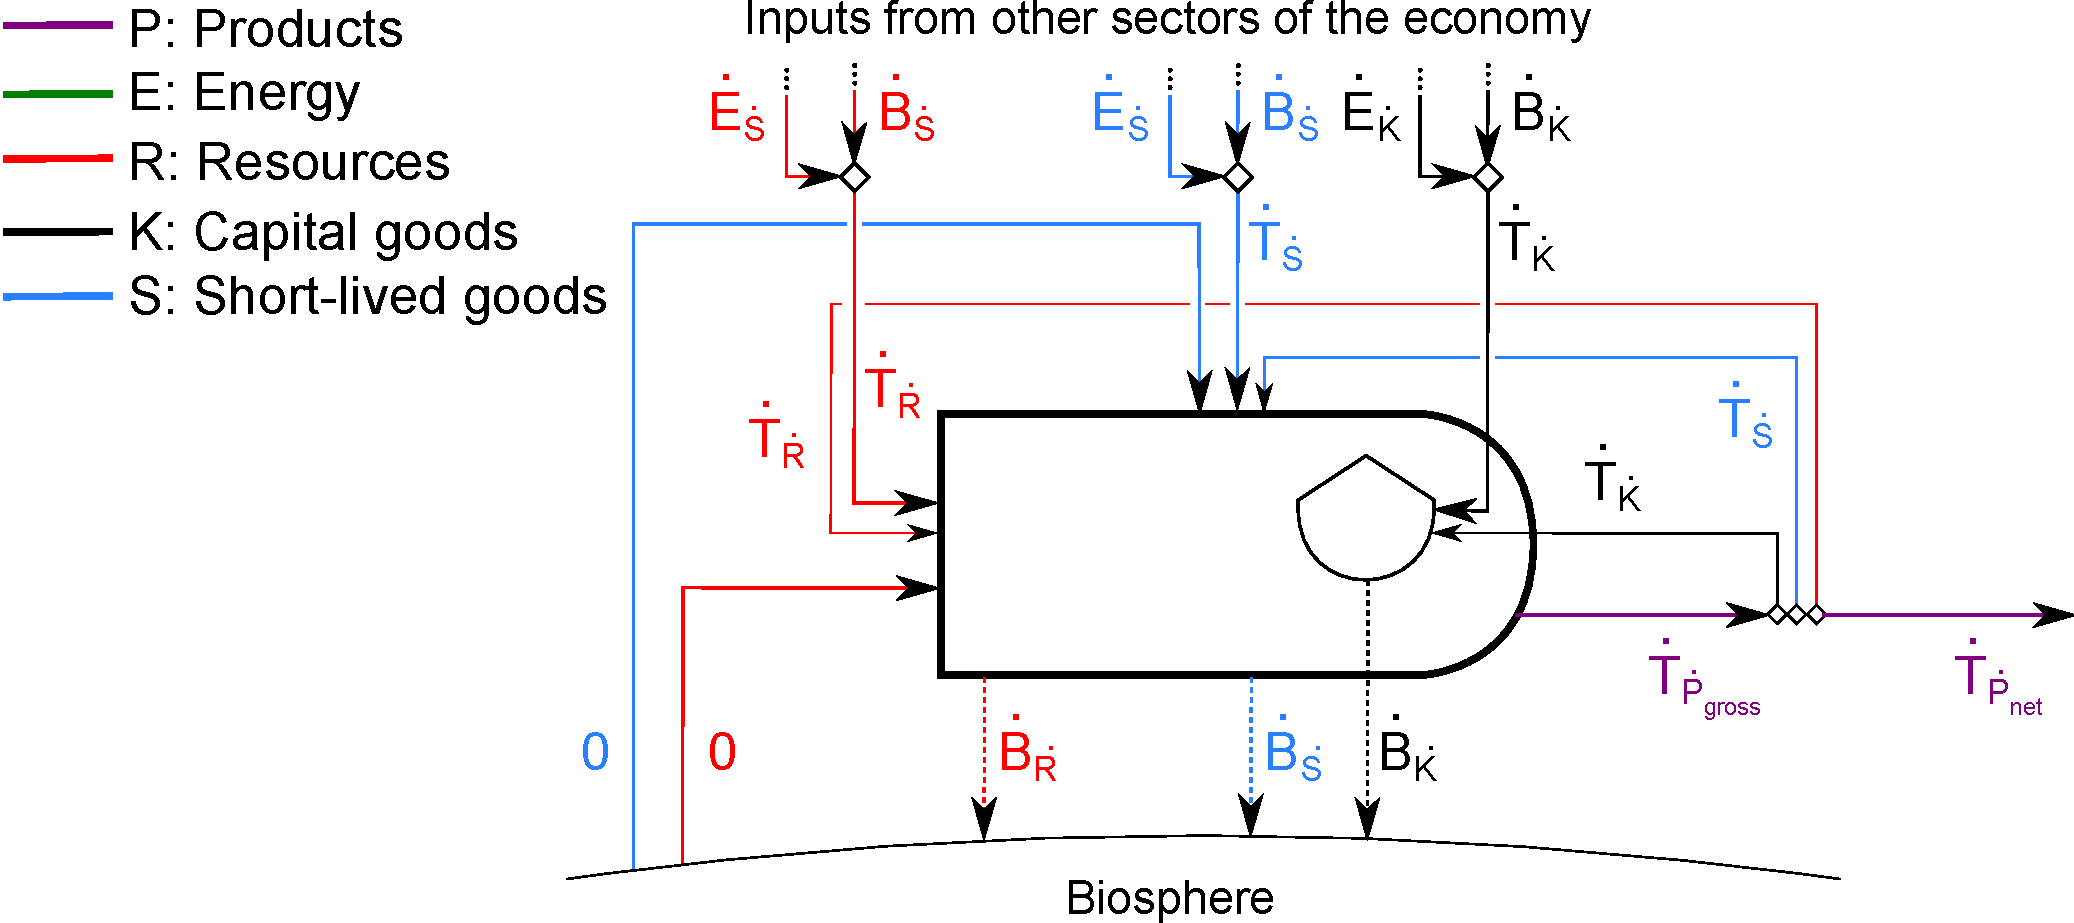
\includegraphics[width=0.8\linewidth]{Part_1/Chapter_Embodied/images/PERKS_basic_unit_embodied_energy_content_auto_ind.pdf}
\caption[Embodied energy flows for the US Automobile Industry]{Embodied energy flows ($\dot{B}$) for the US Automobile Industry using data from XXXX.}
\label{fig:PERKS_embodied_auto}
\end{figure}

Historically, very few estimates of embodied energy of automobiles have been made.
In 1973, Berry and Fels, used a process-based analysis 
(rather an Input-Output analysis),
to find that the energy cost of automobile 
manufacturing\footnote{The ``energy cost'' estimated 
by Berry and Fels is the 
energy embodied in a single automobile. 
The ``energy cost'' (in kW-hr/automobile) multiplied by the 
the production rate (in autmobiles/year) gives the rate of gross embodied
energy outflow in the product stream of the auto sector ($\dot{B}_{\dot{P}_{gross}}$).
A limitation of the process-based approach employed by Berry and Fels
is trucation error for upstream energy demand. 
See Section~\ref{sec:hybrid} for details.
}
in the U.S.\ was 37,275~kW-hr = 134~GJ~(10$^9$~J) 
per vehicle.\cite[Table~2]{Berry:1973vo}

Two decades later in 1995, Stodolsky et al.\ estimated the energy consumed in materials and 
manufacturing automobiles to be 79~GJ per vehicle for a conventional automobile and 66~GJ per vehicle
for an aluminum intensive vehicle, both under a maximum-recycling
scenario.\cite[p.11]{Stodolsky1995}. 
Three years later, MacLean and Lave estimated the the embodied energy
for an automobile to be 113.6~MBtu = 120~GJ per 
vehicle~\cite[Table~1]{MacLean1998}, which they compare with
contemporaneous estimates from Sullivan of 81~GJ per 
vehicle~\cite{Sullivan1995} and Volkswagen of 62~GJ
per vehicle.~\cite{Schweimer1996}

**** MCD---discuss variation in estimates (Berry and Fels uncertainty
10\%) and break out into direct and upstream 
(Berry and Fels Table 2, MacLean Figure 2). ****

Estimates of vehicle embodied energy are related 
to contemporary debates on whether 
Electric Vehicles (EVs) reduce CO$_2$ emissions
relative to Internal Combustion Vehicles (ICVs),
insofar as embodied energy includes upstream supply chain energy consumption,
a major contributor to both EV and ICV lifecycle emissions.
Although EVs have no direct emissions during operation,
accounting for the upstream energy consumed in generating electicty, 
the manufacture of batteries, 
and the production of lightweight materials 
(employed to offset the weight of EV battery packs)
leads to significantly increased lifecycle emissions.
Many studies find that negligible or negative emissions
savings are achieved by EVs.\cite{Anair:2012aa, Hawkins2012,zehner2013unclean}


%%%%%%%%%% Embodied Energy: Summary %%%%%%%%%%
\section{Summary}
\label{sec:embodied_energy_summary}
%%%%%%%%%%


\bibliographystyle{unsrt}
\bibliography{../../EROI_review_v2}


% Always give a unique label
% and use \ref{<label>} for cross-references
% and \cite{<label>} for bibliographic references
% use \sectionmark{}
% to alter or adjust the section heading in the running head
%% Instead of simply listing headings of different levels we recommend to let every heading be followed by at least a short passage of text. Furtheron please use the \LaTeX\ automatism for all your cross-references and citations.

%% Please note that the first line of text that follows a heading is not indented, whereas the first lines of all sequent paragraphs are.

%% Use the standard \verb|equation| environment to typeset your equations, e.g.
%
%% \begin{equation}
%% a \times b = c\;,
%% \end{equation}
%
%% however, for multiline equations we recommend to use the \verb|eqnarray|
%% environment\footnote{In physics texts please activate the class option \texttt{vecphys} to depict your vectors in \textbf{\itshape boldface-italic} type - as is customary for a wide range of physical jects.}.
%% \begin{eqnarray}
%% a \times b = c \nonumber\\
%% \vec{a} \cdot \vec{b}=\vec{c}
%% \label{eq:01}
%% \end{eqnarray}

%% \section{section Heading}
%% \label{sec:2}
%% Instead of simply listing headings of different levels we recommend to let every heading be followed by at least a short passage of text. Furtheron please use the \LaTeX\ automatism for all your cross-references\index{cross-references} and citations\index{citations} as has already been described in Sect.~\ref{sec:2}.

%% \begin{quotation}
%% Please do not use quotation marks when quoting texts! Simply use the \verb|quotation| environment -- it will automatically render Springer's preferred layout.
%% \end{quotation}


%% \section{section Heading}
%% Instead of simply listing headings of different levels we recommend to let every heading be followed by at least a short passage of text. Furtheron please use the \LaTeX\ automatism for all your cross-references and citations as has already been described in Sect.~\ref{sec:2}, see also Fig.~\ref{fig:1}\footnote{If you copy text passages, figures, or tables from other works, you must obtain \textit{permission} from the copyright holder (usually the original publisher). Please enclose the signed permission with the manucript. The sources\index{permission to print} must be acknowledged either in the captions, as footnotes or in a separate section of the book.}

%% Please note that the first line of text that follows a heading is not indented, whereas the first lines of all sequent paragraphs are.

% For figures use
%
%% \begin{figure}[b]
%% \sidecaption
% Use the relevant command for your figure-insertion program
% to insert the figure file.
% For example, with the option graphics use
%% \includegraphics[scale=.65]{figure}
%
% If not, use
%\picplace{5cm}{2cm} % Give the correct figure height and width in cm
%
%% \caption{If the width of the figure is less than 7.8 cm use the \texttt{sidecapion} command to flush the caption on the left side of the page. If the figure is positioned at the top of the page, align the sidecaption with the top of the figure -- to achieve this you simply need to use the optional argument \texttt{[t]} with the \texttt{sidecaption} command}
%% \label{fig:1}       % Give a unique label
%% \end{figure}


%% \paragraph{Paragraph Heading} %
%% Instead of simply listing headings of different levels we recommend to let every heading be followed by at least a short passage of text. Furtheron please use the \LaTeX\ automatism for all your cross-references and citations as has already been described in Sect.~\ref{sec:2}.

%% Please note that the first line of text that follows a heading is not indented, whereas the first lines of all sequent paragraphs are.

%% For typesetting numbered lists we recommend to use the \verb|enumerate| environment -- it will automatically render Springer's preferred layout.

%% \begin{enumerate}
%% \item{Livelihood and survival mobility are oftentimes coutcomes of uneven socioeconomic development.}
%% \begin{enumerate}
%% \item{Livelihood and survival mobility are oftentimes coutcomes of uneven socioeconomic development.}
%% \item{Livelihood and survival mobility are oftentimes coutcomes of uneven socioeconomic development.}
%% \end{enumerate}
%% \item{Livelihood and survival mobility are oftentimes coutcomes of uneven socioeconomic development.}
%% \end{enumerate}


%% \paragraph{paragraph Heading} In order to avoid simply listing headings of different levels we recommend to let every heading be followed by at least a short passage of text. Use the \LaTeX\ automatism for all your cross-references and citations as has already been described in Sect.~\ref{sec:2}, see also Fig.~\ref{fig:2}.

%% Please note that the first line of text that follows a heading is not indented, whereas the first lines of all sequent paragraphs are.

%% For unnumbered list we recommend to use the \verb|itemize| environment -- it will automatically render Springer's preferred layout.

%% \begin{itemize}
%% \item{Livelihood and survival mobility are oftentimes coutcomes of uneven socioeconomic development, cf. Table~\ref{tab:1}.}
%% \begin{itemize}
%% \item{Livelihood and survival mobility are oftentimes coutcomes of uneven socioeconomic development.}
%% \item{Livelihood and survival mobility are oftentimes coutcomes of uneven socioeconomic development.}
%% \end{itemize}
%% \item{Livelihood and survival mobility are oftentimes coutcomes of uneven socioeconomic development.}
%% \end{itemize}

%% \begin{figure}[t]
%% \sidecaption[t]
% Use the relevant command for your figure-insertion program
% to insert the figure file.
% For example, with the option graphics use
%% \includegraphics[scale=.65]{figure}
%
% If not, use
%\picplace{5cm}{2cm} % Give the correct figure height and width in cm
%
%% \caption{Please write your figure caption here}
%% \label{fig:2}       % Give a unique label
%% \end{figure}

%% \runinhead{Run-in Heading Boldface Version} Use the \LaTeX\ automatism for all your cross-references and citations as has already been described in Sect.~\ref{sec:2}.

%% \runinhead{Run-in Heading Italic Version} Use the \LaTeX\ automatism for all your cross-refer\-ences and citations as has already been described in Sect.~\ref{sec:2}\index{paragraph}.
% Use the \index{} command to code your index words
%
% For tables use
%
%% \begin{table}
%% \caption{Please write your table caption here}
%% \label{tab:1}       % Give a unique label
%
% For LaTeX tables use
%
%% \begin{tabular}{p{2cm}p{2.4cm}p{2cm}p{4.9cm}}
%% \hline\noalign{\smallskip}
%% Classes & class & Length & Action Mechanism  \\
%% \noalign{\smallskip}\svhline\noalign{\smallskip}
%% Translation & mRNA$^a$  & 22 (19--25) & Translation repression, mRNA cleavage\\
%% Translation & mRNA cleavage & 21 & mRNA cleavage\\
%% Translation & mRNA  & 21--22 & mRNA cleavage\\
%%Translation & mRNA  & 24--26 & Histone and DNA Modification\\
%%\noalign{\smallskip}\hline\noalign{\smallskip}
%%\end{tabular}
%%$^a$ Table foot note (with superscript)
%%\end{table}
%
%% \section{Section Heading}
%%\label{sec:3}
% Always give a unique label
% and use \ref{<label>} for cross-references
% and \cite{<label>} for bibliographic references
% use \sectionmark{}
% to alter or adjust the section heading in the running head
%% Instead of simply listing headings of different levels we recommend to let every heading be followed by at least a short passage of text. Furtheron please use the \LaTeX\ automatism for all your cross-references and citations as has already been described in Sect.~\ref{sec:2}.

%% Please note that the first line of text that follows a heading is not indented, whereas the first lines of all sequent paragraphs are.

%%If you want to list definitions or the like we recommend to use the Springer-enhanced \verb|description| environment -- it will automatically render Springer's preferred layout.

%%\begin{description}[Type 1]
%%\item[Type 1]{That addresses central themes pertainng to migration, health, and disease. In Sect.~\ref{sec:1}, Wilson discusses the role of human migration in infectious disease distributions and patterns.}
%%\item[Type 2]{That addresses central themes pertainng to migration, health, and disease. In Sect.~\ref{sec:2}, Wilson discusses the role of human migration in infectious disease distributions and patterns.}
%%\end{description}

%%\section{section Heading} %
%% In order to avoid simply listing headings of different levels we recommend to let every heading be followed by at least a short passage of text. Use the \LaTeX\ automatism for all your cross-references and citations citations as has already been described in Sect.~\ref{sec:2}.

%% Please note that the first line of text that follows a heading is not indented, whereas the first lines of all sequent paragraphs are.

%% \begin{svgraybox}
%% If you want to emphasize complete paragraphs of texts we recommend to use the newly defined Springer class option \verb|graybox| and the newly defined environment \verb|svgraybox|. This will produce a 15 percent screened box 'behind' your text.

%% If you want to emphasize complete paragraphs of texts we recommend to use the newly defined Springer class option and environment \verb|svgraybox|. This will produce a 15 percent screened box 'behind' your text.
%% \end{svgraybox}


%% \section{section Heading}
%%Instead of simply listing headings of different levels we recommend to let every heading be followed by at least a short passage of text. Furtheron please use the \LaTeX\ automatism for all your cross-references and citations as has already been described in Sect.~\ref{sec:2}.

%% Please note that the first line of text that follows a heading is not indented, whereas the first lines of all sequent paragraphs are.

%% \begin{theorem}
%% Theorem text goes here.
%% \end{theorem}
%
% or
%
%% \begin{definition}
%% Definition text goes here.
%% \end{definition}

%% \begin{proof}
%\smartqed
%% Proof text goes here.
%% \qed
%% \end{proof}

%%\paragraph{Paragraph Heading} %
%% Instead of simply listing headings of different levels we recommend to let every heading be followed by at least a short passage of text. Furtheron please use the \LaTeX\ automatism for all your cross-references and citations as has already been described in Sect.~\ref{sec:2}.

%% Note that the first line of text that follows a heading is not indented, whereas the first lines of all subsequent paragraphs are.
%
% For built-in environments use
%
%%\begin{theorem}
%%Theorem text goes here.
%%\end{theorem}
%
%%\begin{definition}
%%Definition text goes here.
%%\end{definition}
%
%%\begin{proof}
%%\smartqed
%% Proof text goes here.
%%\qed
%%\end{proof}
%
%% \begin{acknowledgement}
%% If you want to include acknowledgments of assistance and the like at the end of an individual chapter please use the \verb|acknowledgement| environment -- it will automatically render Springer's preferred layout.
%% \end{acknowledgement}
%
%% \section*{Appendix}
%% \addcontentsline{toc}{section}{Appendix}
%
%% When placed at the end of a chapter or contribution (as opposed to at the end of the book), the numbering of tables, figures, and equations in the appendix section continues on from that in the main text. Hence please \textit{do not} use the \verb|appendix| command when writing an appendix at the end of your chapter or contribution. If there is only one the appendix is designated ``Appendix'', or ``Appendix 1'', or ``Appendix 2'', etc. if there is more than one.

%% \begin{equation}
%% a \times b = c
%% \end{equation}
% Problems or Exercises should be sorted chapterwise
%% \section*{Problems}
%% \addcontentsline{toc}{section}{Problems}
%
% Use the following environment.
% Don't forget to label each problem;
% the label is needed for the solutions' environment
%% \begin{prob}
%% \label{prob1}
%% A given problem or Excercise is described here. The
%% problem is described here. The problem is described here.
%% \end{prob}

%% \begin{prob}
%% \label{prob2}
%% \textbf{Problem Heading}\\
%% (a) The first part of the problem is described here.\\
%% (b) The second part of the problem is described here.
%% \end{prob}


